%  LaTeX support: latex@mdpi.com
%  For support, please attach all files needed for compiling as well as the log file, and specify your operating system, LaTeX version, and LaTeX editor.

%=================================================================
\documentclass[sensors,article,submit,moreauthors]{Definitions/mdpi}

%=================================================================
% MDPI internal commands - do not modify
\firstpage{1}
\makeatletter
\setcounter{page}{\@firstpage}
\makeatother
\pubvolume{1}
\issuenum{1}
\articlenumber{0}
\pubyear{2026}
\copyrightyear{2026}
\datereceived{}
\daterevised{}
\dateaccepted{}
\datepublished{}

%=================================================================
% Add packages and commands here. The following packages are loaded in our class file: fontenc, inputenc, calc, indentfirst, fancyhdr, graphicx, epstopdf, lastpage, ifthen, float, amsmath, amssymb, lineno, setspace, enumitem, mathpazo, booktabs, titlesec, etoolbox, tabto, xcolor, colortbl, soul, multirow, microtype, tikz, totcount, changepage, attrib, upgreek, array, tabularx, pbox, ragged2e, tocloft, marginnote, marginfix, enotez, amsthm, natbib, hyperref, cleveref, scrextend, url, geometry, newfloat, caption, draftwatermark, seqsplit
% cleveref: load \crefname definitions after \begin{document}

\usepackage{subcaption}  %% subtable environment for split tables (loaded after MDPI class)

%=================================================================
% Title (Capitalized)
\Title{TP-Net: Self-Supervised Pretrained Network Traffic Representations for Few-Shot Threat Detection in IoT and Sensor Networks}

% Authors
\Author{Xi Yao $^{1}$, Yan Feng $^{1,}$* and Qianchu Wang $^{1}$}

% MDPI internal command: Authors for metadata in PDF
\AuthorNames{Xi Yao, Yan Feng and Qianchu Wang}

% Affiliations
\address{%
$^{1}$ \quad School of Information Science and Technology, Tibet University, Najin Road, Lhasa 850000, China; 13574913636@163.com (X.Y.); 13518918910@163.com (Y.F.); 2952719824@qq.com (Q.W.)\\
}

% Contact information of the corresponding author
\corres{Correspondence: 13518918910@163.com; Tel.: +86-135-1891-8910 (Y.F.)}

% Abstract
\abstract{With more than 90\% of IoT and sensor-network traffic now encrypted and new attacks emerging weekly, deep-packet inspection and fully supervised classifiers are bottlenecked by label scarcity and encoder-retraining cost at the resource-constrained IoT edge. We argue the operational metric for IoT-edge detection should be how few labels and how much encoder retraining are required to recognise a new attack, not raw full-shot accuracy. TP-Net (Traffic Pretraining Network) couples self-supervised contrastive pretraining with $N$-way $K$-shot evaluation: a four-branch 1D-CNN encoder is trained once under SimCLR on packet, burst, flow-statistical, and TLS-handshake features with five traffic-specific augmentations, then frozen at deployment. On three IoT-relevant datasets (CIC-IDS2017, USTC-TFC2016, ISCX-VPN2016), TP-Net SSL ProtoNet lifts 5-shot accuracy over a random encoder by $+13.14/+7.76/+4.11$ pp and reaches $99.3\%/72.9\%/100\%$ on completely unseen novel-class attacks. On fully encrypted DoHBrw-2020 SSL gains $+28.66$ pp over no-pretrain. Under the same per-episode linear head, TP-Net's SSL encoder places in the competitive-middle band, trailing the strongest fully-trained supervised model (YaTC, 50 ep) by at most $9.75$ pp without any encoder fine-tuning. Augmentation strength must adapt to task complexity, overturning the canonical SimCLR ``stronger-is-better'' rule on IoT traffic. TP-Net's primary value is a 5-alert, no-finetune, hour-level deployment path for novel encrypted attacks at the IoT edge.}

% Keywords
\keyword{IoT security; sensor network traffic classification; self-supervised contrastive learning; few-shot learning; novel attack detection; edge computing}

%=================================================================
\renewcommand{\floatpagefraction}{0.95}
\renewcommand{\topfraction}{0.95}
\renewcommand{\bottomfraction}{0.95}
\renewcommand{\textfraction}{0.02}
\usepackage{longtable}
\begin{document}

%% ===============================================================
%% Main body
%% ===============================================================

%% ----------------------------------------------------------------
\section{Introduction}
%% ----------------------------------------------------------------

\subsection{Background and motivation}

Encrypted traffic now accounts for more than 90\% of network traffic \cite{cisco2024threat}. Attackers have accordingly migrated command-and-control (C2) communications and malicious payloads to TLS, DoH, QUIC, and other encrypted channels. Against these channels, traditional deep-packet-inspection and plaintext-payload solutions such as Snort and Suricata are largely ineffective. Even for traffic that remains partially plaintext, increasingly complex application-layer encapsulation keeps the maintenance cost of DPI prohibitively high.

Behavior-based traffic analysis has therefore become the prevailing direction. By inferring the traffic category from packet-length sequences, burst patterns, flow statistics, and handshake features (e.g., JA3), it is well suited to the dominant case of encrypted traffic, which is the most salient driver of this shift. Representative works in this direction include FS-Net \cite{liu2019fsnet}, YaTC \cite{zhao2023yatc}, ET-BERT \cite{lin2022etbert}, and TFE-GNN \cite{zhang2023tfegnn}; see \cite{dhinakar2026survey} for a survey. These methods, however, generally struggle with novel attacks: new-attack alerts are typically a single digit, making full supervision expensive to label, and the learned features are coupled to the training-set distribution and transfer poorly; traditional architectures further require full retraining, which cannot keep pace with attackers' rapid turnover of C2 domains and payloads. The central methodological challenge posed by these pain points is how to endow a traffic-detection model with both \emph{few-shot} capability and \emph{strong generalization}.

This challenge is particularly acute in IoT and sensor networks, where devices are often deployed in resource-constrained edge environments with limited computational capacity and intermittent connectivity to cloud infrastructure. Unlike general-purpose enterprise traffic, IoT sensor traffic exhibits distinct characteristics: highly periodic telemetry patterns, limited payload diversity, and strict latency requirements for local anomaly detection \cite{liu2025iot}. Recent work has shown that self-supervised embeddings can be made extensible to IoT and wireless sensor networks (WSNs) where resource constraints and new attack surfaces demand lightweight yet semantically enriched intrusion-detection solutions \cite{liu2025iot}. These constraints make the retraining-heavy supervised paradigm of conventional traffic classifiers impractical at the IoT edge, and amplify the value of a pretrained, frozen encoder that can recognise novel threats with only a handful of labelled alerts. TP-Net is designed against this IoT-edge backdrop: a one-time SimCLR pretraining produces a frozen four-branch encoder that runs in real time on commodity gateways, while novel attacks are absorbed by fitting a one-line \texttt{sklearn} LogReg on $K = 5$ support samples without any encoder retraining.

\subsection{Gap with existing work}
\label{sec:gap}

The systematic differences between existing research and the proposed TP-Net (Traffic Pretraining Network) span five dimensions, summarized in Table~\ref{tab:diff}. A core distinction from the ``SSL followed by full supervision'' paradigm (as in ET-BERT) is that, in TP-Net, the encoder is no longer updated after the pretraining stage, and the downstream evaluation is conducted exclusively through $N$-way $K$-shot episodes, forming a complete SSL--few-shot closed loop rather than using SSL merely to accelerate fully supervised training.

\begin{table}[H]
\small
\caption{Five-dimensional comparison of existing work and TP-Net.}
\label{tab:diff}
\begin{adjustwidth}{-\extralength}{0cm}
\begin{tabularx}{\fulllength}{>{\centering\arraybackslash}X>{\centering\arraybackslash}X>{\centering\arraybackslash}X}
\toprule
Dimension & Existing work & TP-Net (this paper)\\
\midrule
Learning paradigm & Fully supervised training & SSL pretraining + few-shot evaluation \\
Novel attack adaptation & Full retraining (hours--days) & 5-shot labeling, hour-level deployment \\
Representation independence & Encoder tightly coupled to head & Frozen encoder, plug-and-play \\
Evaluation protocol & Fixed train/val/test split & $N$-way $K$-shot episode protocol \\
Data augmentation & CV-style flipping/cropping & Five traffic-specific, physically meaningful augmentations \\
\bottomrule
\end{tabularx}
\end{adjustwidth}
\end{table}

\subsection{Contributions}
\label{sec:contrib}

This paper makes three principal contributions, matching the structure of the Abstract.

\medskip

\noindent\textbf{C1: Protocol-fair SOTA comparison under a single frozen-encoder evaluation head.} We deliver a systematic, protocol-fair evaluation against six supervised-traffic baselines (ET-BERT, FS-Net, YaTC, NetConv, NetMamba, TFE-GNN) on three IoT-relevant datasets (CIC-IDS2017, USTC-TFC2016, ISCX-VPN2016), under the \emph{same} per-episode \texttt{sklearn} LogReg ($C = 10^3$) head on $K$ support samples, with a focus on IoT-edge few-shot deployment scenarios. The encoder of every baseline is supervised-trained on the same 20\,k stratified subset for the same 3 supervised epochs, frozen, and evaluated through the same $N$-way $K$-shot episode protocol. To address the natural concern that 3 epochs under-trains the baselines, we additionally re-train the two strongest supervised baselines (YaTC, TFE-GNN) for a full 50 epochs in a \emph{Full-budget sanity check} block. The headline conclusion is robust to baseline training budget: TP-Net SSL FT-Head places in the competitive-middle band on every dataset, trailing the strongest fully-trained supervised model (YaTC, 50 ep) by $6.84$ pp (CIC), $3.70$ pp (USTC) and $9.75$ pp (ISCX).

\medskip

\noindent\textbf{C2: Novel-class and encrypted-only generalization.} We demonstrate that the framework generalises to completely unseen IoT attack classes: CIC 2-class novel reaches $99.3\%$ 5-shot accuracy, and USTC 5-class novel reaches $72.9\%$. Importantly, the same SSL encoder retains its advantage on a fully encrypted IoT workload. On the DoHBrw-2020 DNS-over-HTTPS subset (a common channel for IoT devices to reach C2 servers), TP-Net SSL 2-way 5-shot reaches $0.838$ vs.\ the no-pretrain random encoder's $0.551$ ($+28.66$ pp). This rules out the failure mode in which the SSL gain on the three primary datasets is a side-effect of plaintext payload access.

\medskip

\noindent\textbf{C3: Task-adaptive augmentation strength.} We show that the canonical ``stronger-is-better'' SimCLR augmentation rule \emph{does not transfer to traffic data} unmodified. The optimal preset is task-dependent: \texttt{none} for the 2-class ISCX task, \texttt{medium} for the 10-class CIC task, and \texttt{weak} for the 20-class USTC task. The full $3 \times 4$ ablation (3 datasets $\times$ 4 augmentation presets) is reported in Table~5, and the cross-dataset CKA / transfer matrix is reported in \S4.5.

%% ----------------------------------------------------------------
\section{Related Work}
%% ----------------------------------------------------------------

\subsection{Behavior-based traffic classification, SSL, and FSL background}
\label{sec:behavioral}

Traffic classification has shifted toward behavior-based features because payload parsing is either infeasible or too costly, and encrypted traffic is the most salient driver of this shift. FS-Net \cite{liu2019fsnet} trains an encoder--decoder to reconstruct packet-length sequences; YaTC \cite{zhao2023yatc} applies a Transformer over 2D traffic matrices; ET-BERT \cite{lin2022etbert} performs MLM pretraining within a BERT framework; TFE-GNN \cite{zhang2023tfegnn} uses a graph neural network over burst topology; and NetMamba \cite{wang2024netmamba} introduces a state-space model (Mamba) for long-range dependencies. All of these methods rely on large amounts of labeled data and require retraining to transfer to new attacks.

Self-supervised contrastive learning \cite{lekhac2020contrastive,jing2021ssl,dong2025sslreview} and few-shot learning \cite{wang2020fsl} provide two complementary levers. Contrastive SSL spans three families: \emph{in-batch negatives} (SimCLR \cite{chen2020simclr}, MoCo \cite{he2020moco}), \emph{negative-free bootstrapping} (BYOL \cite{grill2020byol}, SimSiam \cite{chen2021simsiam}), and \emph{reconstructive generative} (MAE \cite{he2022mae}). We adopt SimCLR because in-batch contrast directly models the ``local similarity'' of traffic data (samples from the same application within a batch naturally form clusters), it requires no momentum queue, and its contrastive loss plateaus after epoch 20, avoiding unnecessarily long training. Few-shot learning follows three routes---metric learning (ProtoNet \cite{snell2017protonet}, MatchingNet \cite{vinyals2016matching}), meta-learning (MAML \cite{finn2017maml}), and learnable distance (RelationNet \cite{sung2018relationnet}). We adopt ProtoNet as the default evaluation paradigm because it is parameter-free, deterministic, and naturally compatible with the SSL philosophy of ``learning representations, not classifiers.''

\subsection{SSL / FSL for traffic analysis and the IoT positioning of this work}
\label{sec:trafficssl}

Several recent works apply SSL or few-shot learning to network traffic classification. ET-BERT \cite{lin2022etbert} and Flow-MAE \cite{hang2023flowmae} stop at fully supervised downstream; YaTC, FS-Net, and other representative works all depend on large amounts of labels. Improved paradigms for few-shot encrypted-traffic classification include in-context-learning-based ICT-META \cite{chang2026ictmeta}, contrastive-driven meta-learning \cite{li2025contrastivemeta}, a pretraining--contrastive-learning synergy for few-shot novelty detection \cite{zhao2026pretraincontrast}, payload-free open-set prototype rejection (SepSpace) \cite{qu2026sepSpace}, SSCL-IDS \cite{golchin2024ssclids}, and MAML combined with contrastive learning \cite{jin2025mamlcl}; recent surveys \cite{rahaman2026review,yang2024clidssurvey} characterise this emerging line. Most works focus on a single component (either SSL or FSL alone); a systematic evaluation, under one unified protocol, of the synergy among SSL representations, FSL heads, and traffic-specific augmentations remains limited---the gap that the present work fills.

The closest contemporaneous work is Ben Atitallah et~al.\ \cite{atitallah2024iot}, which combines a Deep Infomax SSL encoder with Prototypical Networks and a downstream Random Forest for IoT malware image classification on MaleVis and WSN-DS. Their line of work shares the SSL + ProtoNet + IoT positioning that motivates TP-Net but differs on three deployment-relevant respects. On the evaluation protocol, Ben Atitallah et~al.\ fine-tune ProtoNet on each few-shot episode, whereas TP-Net keeps the encoder frozen and fits only a one-line \texttt{sklearn} LogReg on $K$ support samples; this avoids the hour-to-day fine-tuning cost that IoT gateways cannot afford. The SSL objective also differs: Deep Infomax maximises mutual information between local and global features, while TP-Net uses SimCLR in-batch contrastive learning that is closer to the closed-form few-shot prototype geometry. Their method processes malware visualisations (grey-scale image renderings of executable bytes) rather than the four-modality traffic-feature inputs (packet, burst, flow statistics, TLS handshake) that TP-Net uses, so the deployment scenarios are complementary rather than overlapping.

Within the IoT and sensor-network sub-community the line is especially active. Liu \& Guo \cite{liu2025iot} recently showed that self-supervised semantic embeddings extend to IoT and WSN intrusion detection, achieving $98.5\%$ accuracy on a 100K-record China Mobile dataset and motivating ``lightweight yet semantically enriched'' IDS for resource-constrained WSNs. Lu et al.\ \cite{lu2026cdtf} proposed the Contrastive Dual-Task Framework (CDTF), combining supervised-triplet pretraining with self-supervised dynamic-burst-masking, evaluated on seven public IoT datasets in MEC environments ($+4.61$ pp Precision under few-shot). These works share TP-Net's high-level motivation (frozen-encoder few-shot detection for encrypted IoT traffic) but differ from TP-Net on two protocol-level respects. On the pretraining objective, CDTF uses a hybrid supervised + self-supervised objective that requires base-class labels, while TP-Net uses pure-SSL SimCLR with zero base-class labels. On the evaluation protocol, CDTF is evaluated under standard supervised fine-tuning, while TP-Net is evaluated under a strictly frozen-encoder $N$-way $K$-shot episode protocol that more faithfully reflects the IoT-edge deployment scenario where encoder retraining is impractical. The present work therefore complements the IoT SSL/FSL line by quantifying what a strictly frozen-encoder, pure-SSL pipeline can achieve on IoT-relevant traffic with only $K = 5$ labelled alerts per novel class.

%% ----------------------------------------------------------------
\section{Materials and Methods}
%% ----------------------------------------------------------------

The overall architecture of TP-Net is illustrated in Figure~\ref{fig:framework}. The pipeline proceeds in four stages. The input flow (four-dimensional features) is fed through a four-branch encoder to extract a 128-dimensional embedding. Two branches then follow: offline SSL pretraining (one-shot) and online few-shot evaluation with a frozen encoder (5 labels per new attack).

\begin{figure}[!htbp]
\begin{adjustwidth}{-\extralength}{0cm}
\centering
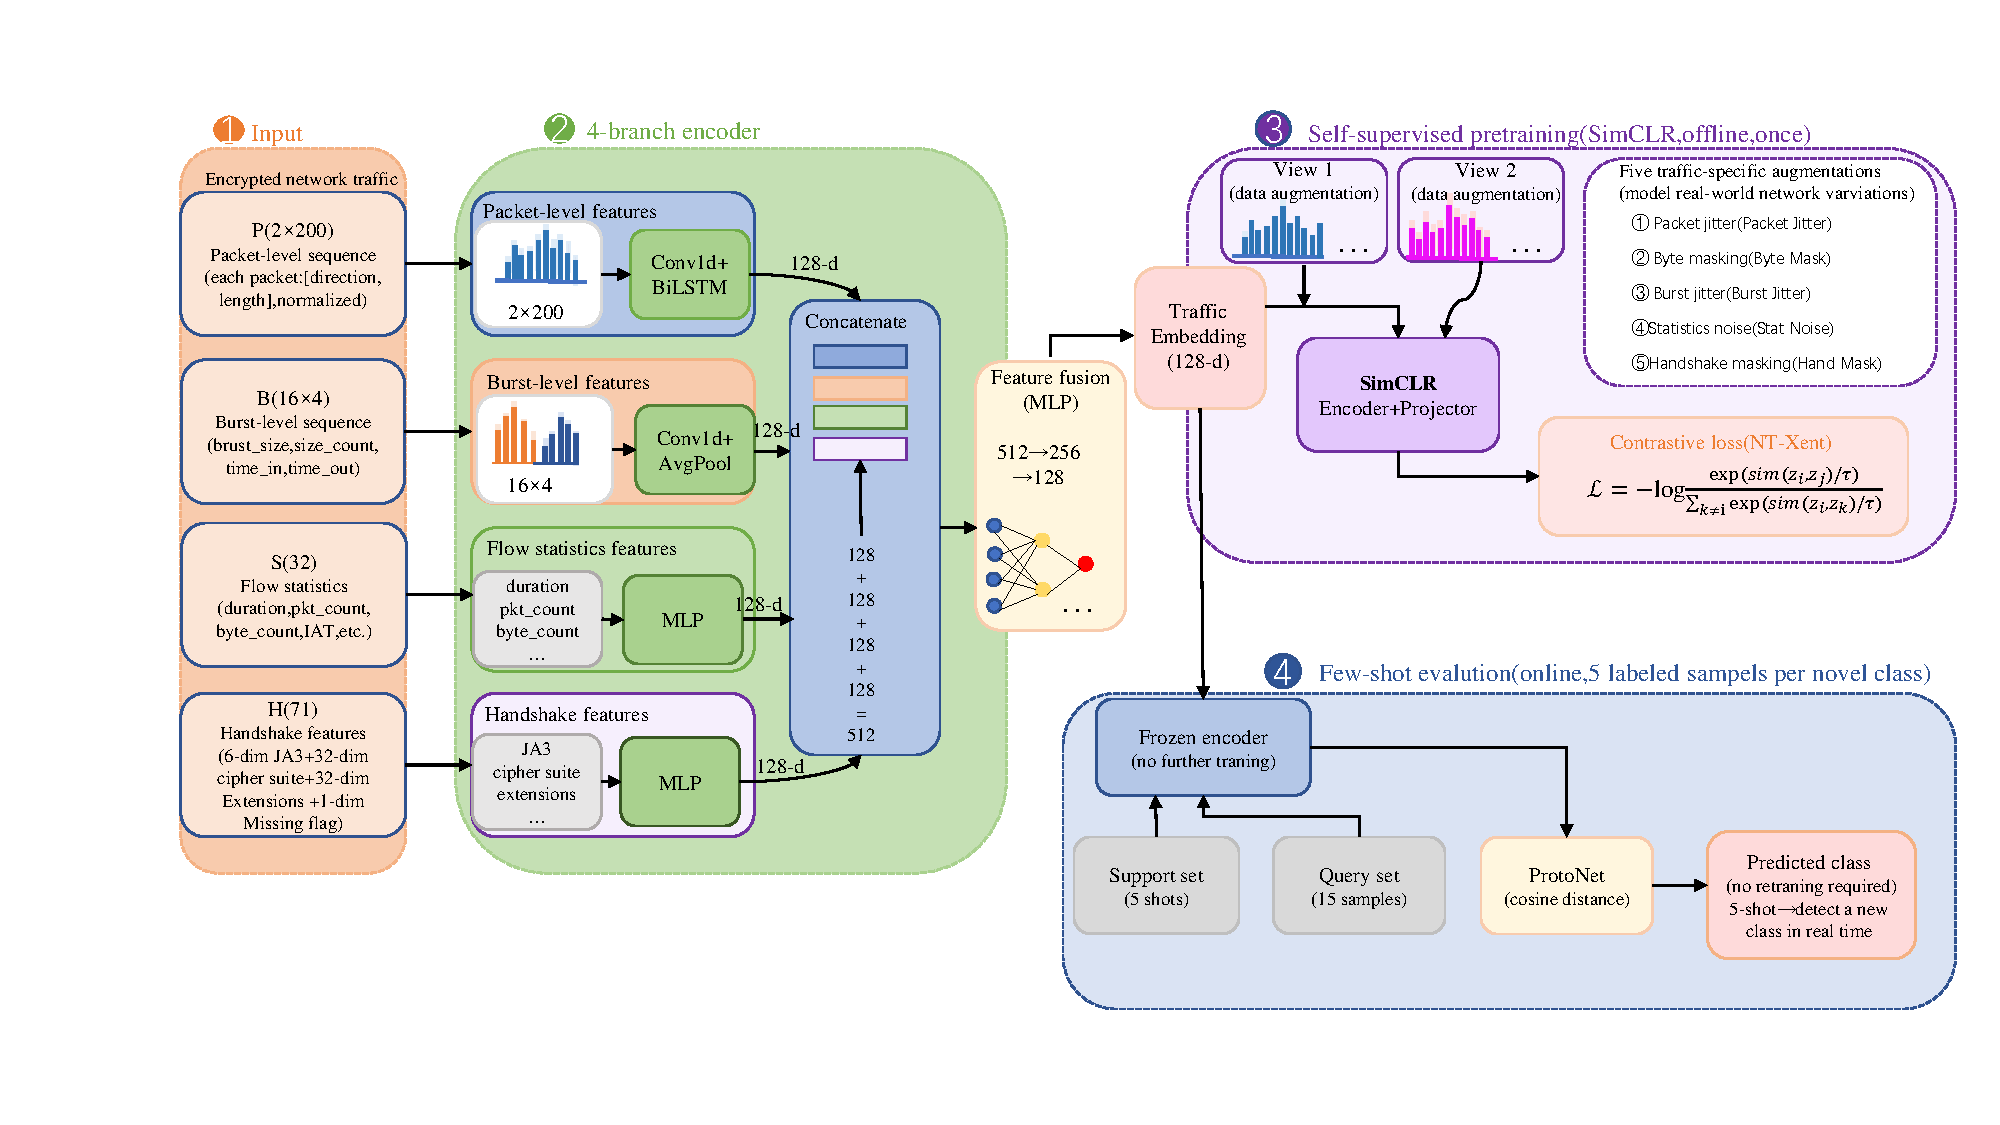
\includegraphics[width=\fulllength]{figures/fig1_framework.pdf}
\label{fig:framework}
\end{adjustwidth}
\caption{Overall architecture of TP-Net.}
\end{figure}

\subsection{Threat model and deployment assumptions}
\label{sec:threatmodel}

We consider a single-tenant IoT-edge gateway that sits at the boundary between an (possibly encrypted) local sensor network and the wider internet. Three operational conditions shape the threat model.

Regarding adversary capability, the attacker controls the contents of the traffic seen at the gateway but not the gateway itself. Concretely, the attacker can (i) craft arbitrary payloads and packet sequences within the application-layer protocol, (ii) tunnel malicious traffic over encrypted channels such as TLS, DoH, or QUIC, and (iii) rotate C2 domains and TLS fingerprints at a faster cadence than the operator can collect labelled samples. The attacker does \emph{not} have direct access to the gateway hardware, the pretrained encoder, or the operator's labelling pipeline.

The defender operates a trusted gateway with limited but adequate computational resources: a commodity IoT-class CPU suffices for one forward pass of the four-branch 1D-CNN (millisecond-level latency per flow) and for fitting a one-line \texttt{sklearn} LogReg on $K$ support samples per class. The gateway can collect a small number (we assume $K \in \{1, 2, 3, 5, 10\}$) of operator-confirmed alerts per novel attack class without retraining the encoder. We assume the SSL pretraining corpus is assembled offline from sources the operator trusts (the captured background traffic of the same deployment plus any relevant public datasets) and is not adversarially poisoned at the point of pretraining; an extension to certified-robust SSL pretraining is left to future work.

We do not consider adversarial packet-length perturbations, feature obfuscation that breaks our four-modality pipeline, or firmware compromise of the gateway. Robustness to such conditions requires dedicated defences (e.g.\ adversarial training, encrypted-traffic anomaly detection) that are orthogonal to the SSL + few-shot design studied here.

\subsection{Problem definition and architecture}
\label{sec:problemdef}

We represent a single encrypted network flow using four feature modalities: $P \in \mathbb{R}^{2 \times 200}$ (packet sequence, each packet binarised as [direction, length]), $B \in \mathbb{R}^{16 \times 4}$ (burst [size, time]), $S \in \mathbb{R}^{32}$ (flow statistics, IAT, byte/pkt count), and $H \in \mathbb{R}^{71}$ (handshake: 6-d JA3 + 32-d cipher suites + 32-d extensions + 1-d miss flag). The objective is to learn an encoder $f_\theta(\cdot)$ such that flows of the same class are close in the embedding space and only $K$ labelled samples are required to classify a novel attack.

Figure~\ref{fig:encoder} details the four-branch encoder: each branch processes one modality independently, and a fusion MLP concatenates and integrates the four branch outputs into a 128-D embedding.

\begin{figure}[!htbp]
\centering
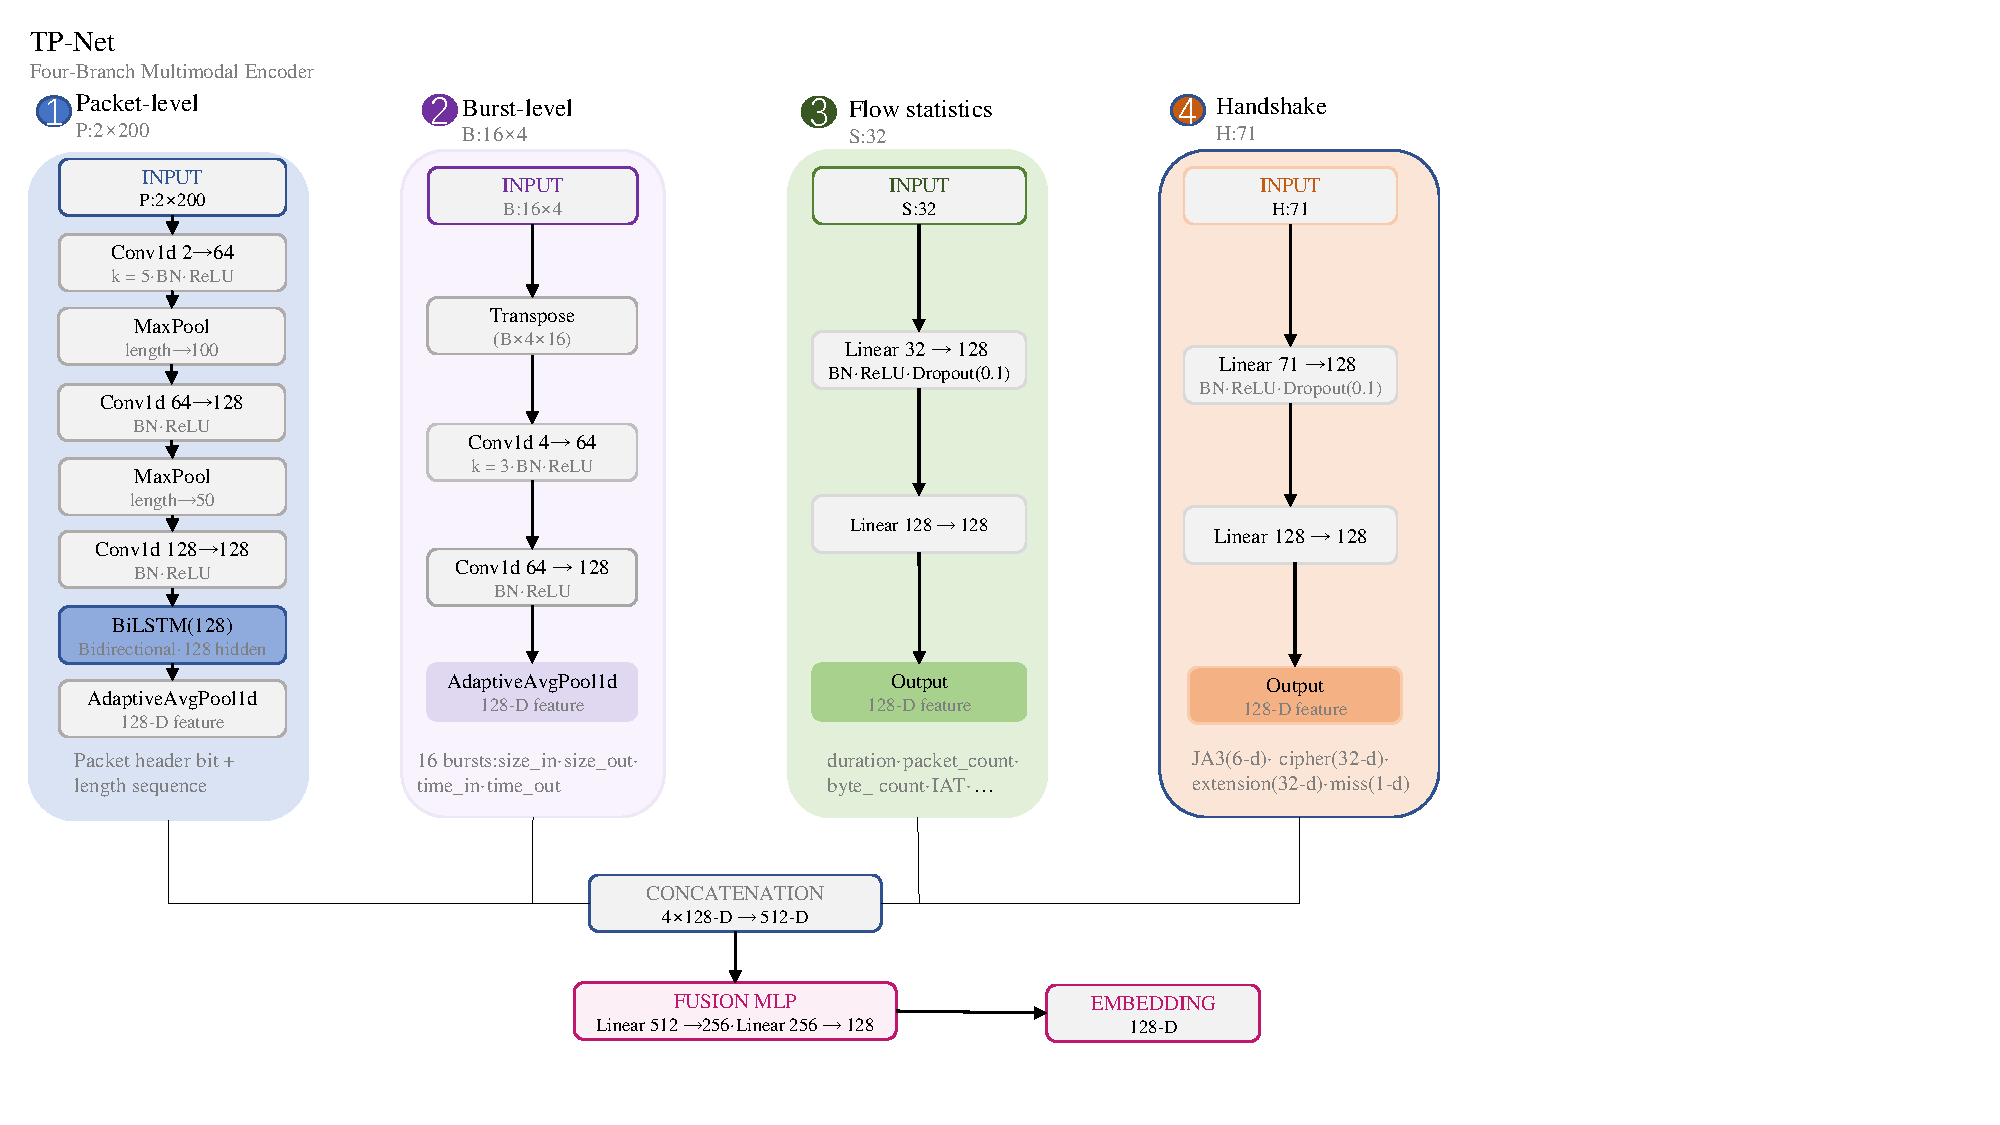
\includegraphics[width=\textwidth, trim=0 0 250 0, clip]{figures/fig2_encoder.pdf}
\caption{Detailed structure of the four-branch encoder.}
\label{fig:encoder}
\end{figure}

\subsection{Augmentation and SSL pretraining}
\label{sec:aug}
\label{sec:ssltrain}

Figure~\ref{fig:aug} visualizes the five traffic-specific augmentations proposed in this work. Each augmentation simulates a real-world network perturbation. The \texttt{none} preset zeroes all augmentation probabilities; although the positive pair then degenerates to an identity mapping, the $2(B-1)$ negative pairs in the batch and the random subsampling performed at data-loading time still provide a discriminative signal. The empirical benefit of \texttt{none} on ISCX is reported in Table~\ref{tab:augabl}.

\begin{figure}[!htbp]
\centering
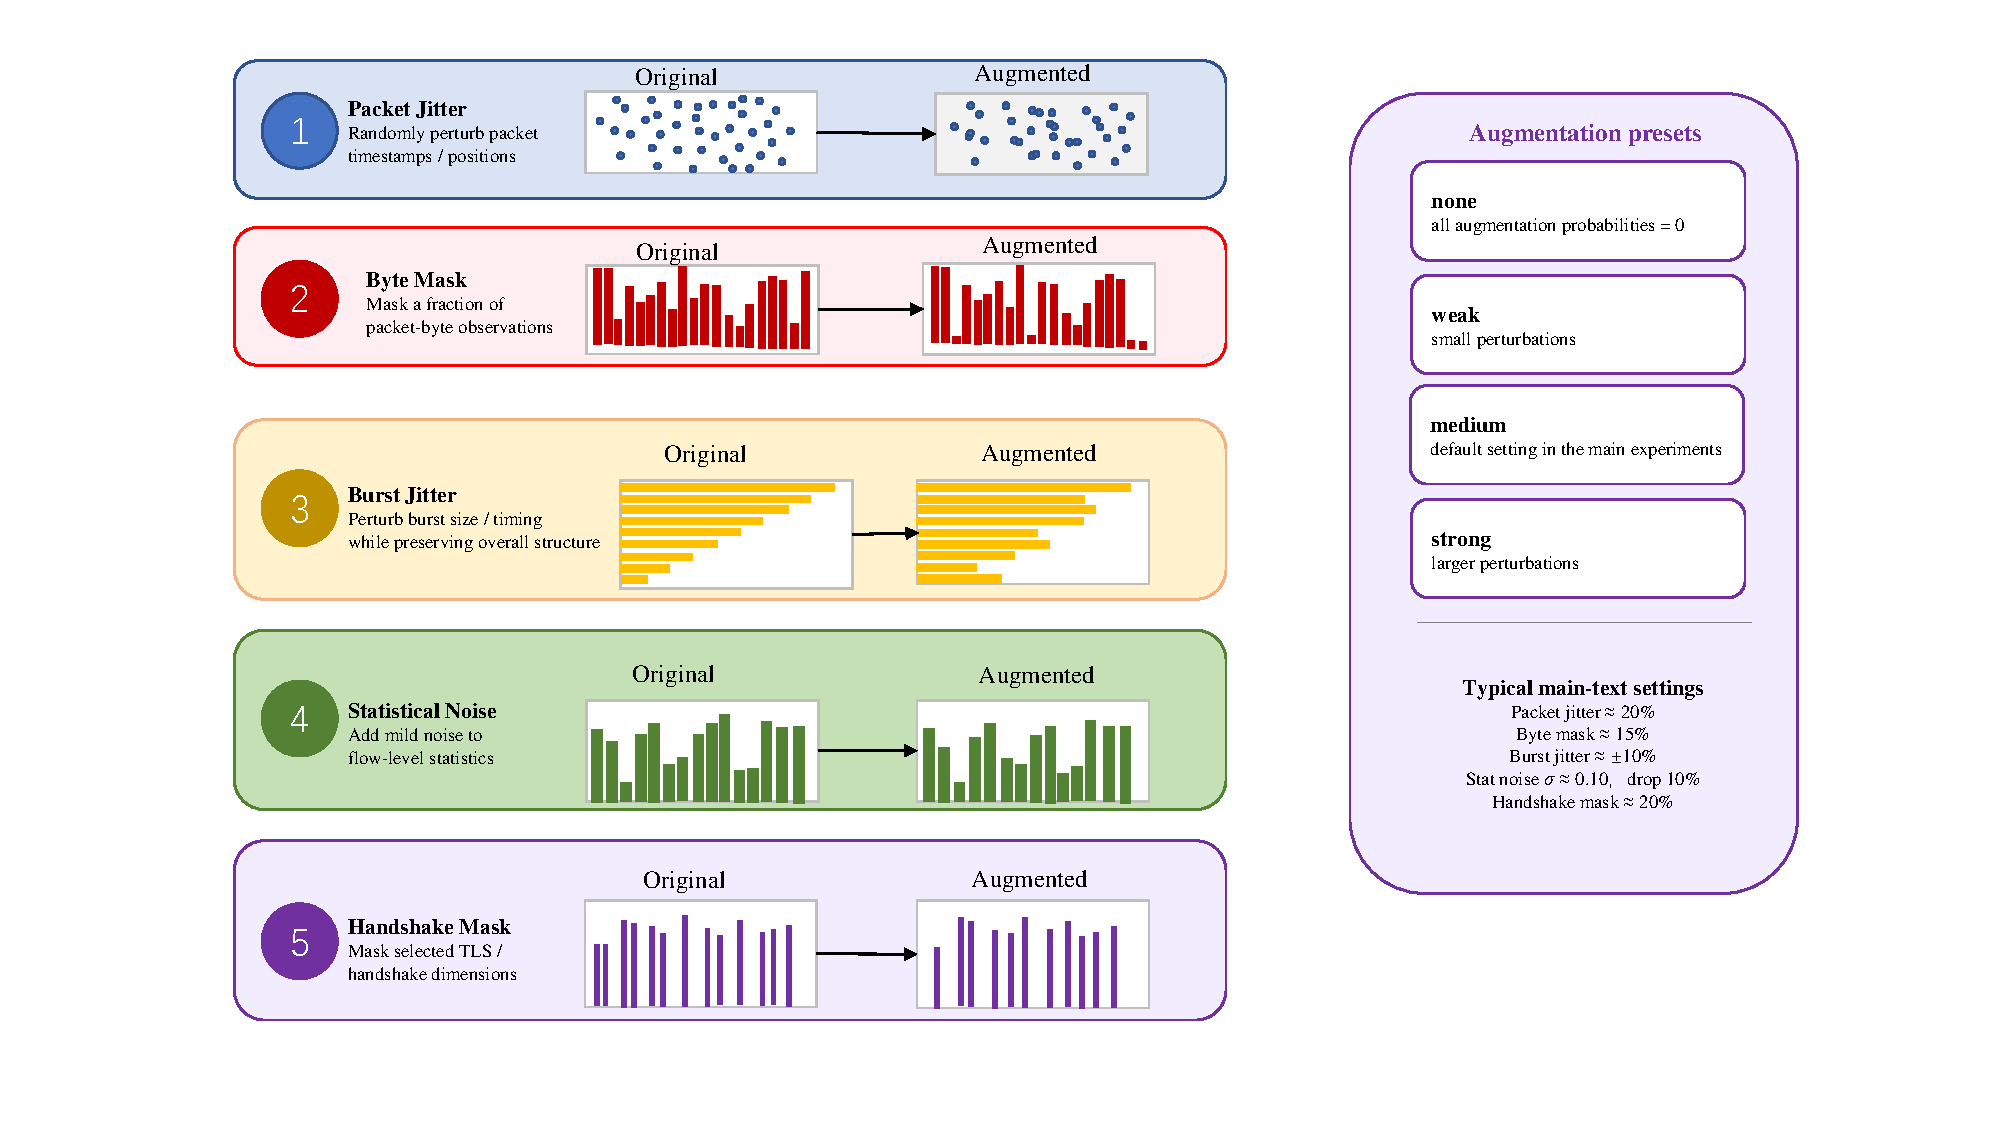
\includegraphics[width=\textwidth]{figures/fig3_augmentation.pdf}
\caption{Schematic of the five traffic-specific augmentations (with the four intensity presets \texttt{none}/\texttt{weak}/\texttt{medium}/\texttt{strong}).}
\label{fig:aug}
\end{figure}

The contrastive loss is the standard NT-Xent (Eq.~\ref{eq:ntxent}, $\tau=0.1$); for each sample $x$ in the batch, two augmentations $x_i$, $x_j$ form the positive pair and all other in-batch samples serve as negatives. The 128-D encoder output is projected into the contrastive space through a 2-layer MLP ($128 \to 128 \to 128$) used only during SSL and discarded at evaluation time. Optimization uses AdamW with $\text{lr} = 3 \times 10^{-4}$, weight decay $1 \times 10^{-4}$, cosine schedule, batch size 256; MoCo additionally maintains a 4096-entry momentum queue. Training stops after 30--50 epochs because the NT-Xent loss plateaus beyond epoch 20. Moderate temperature $\tau = 0.1$ suffices because traffic data has small intra-class and large inter-class variance.

\begin{equation}
\label{eq:ntxent}
\mathcal{L}_{\text{NT-Xent}} = -\log \frac{\exp(\text{sim}(z_i, z_j)/\tau)}{\sum_{k \neq i} \exp(\text{sim}(z_i, z_k)/\tau)}
\end{equation}

\subsection{Few-shot and novel-class evaluation protocols}
\label{sec:fslproto}
\label{sec:sslalgo}

In deployment, novel attacks have only a handful of labelled samples (5--50); the conventional train/val/test split cannot faithfully reflect this ``small-sample'' scenario. The $N$-way $K$-shot episode protocol is therefore closer to operational needs. At each round, $N$ classes are sampled uniformly at random; for each, $K$ support and $Q$ query samples are drawn, the encoder computes a prototype from the support set, and accuracy is measured on the queries (Figure~\ref{fig:protonet}, Eq.~\ref{eq:protonet}). We adopt the cosine-distance variant of ProtoNet ($d = 1 - \cos$) for stability at small $K$; MatchingNet is also evaluated as a comparator (see~\S\ref{sec:mainexp}).

\begin{figure}[!htbp]
\centering
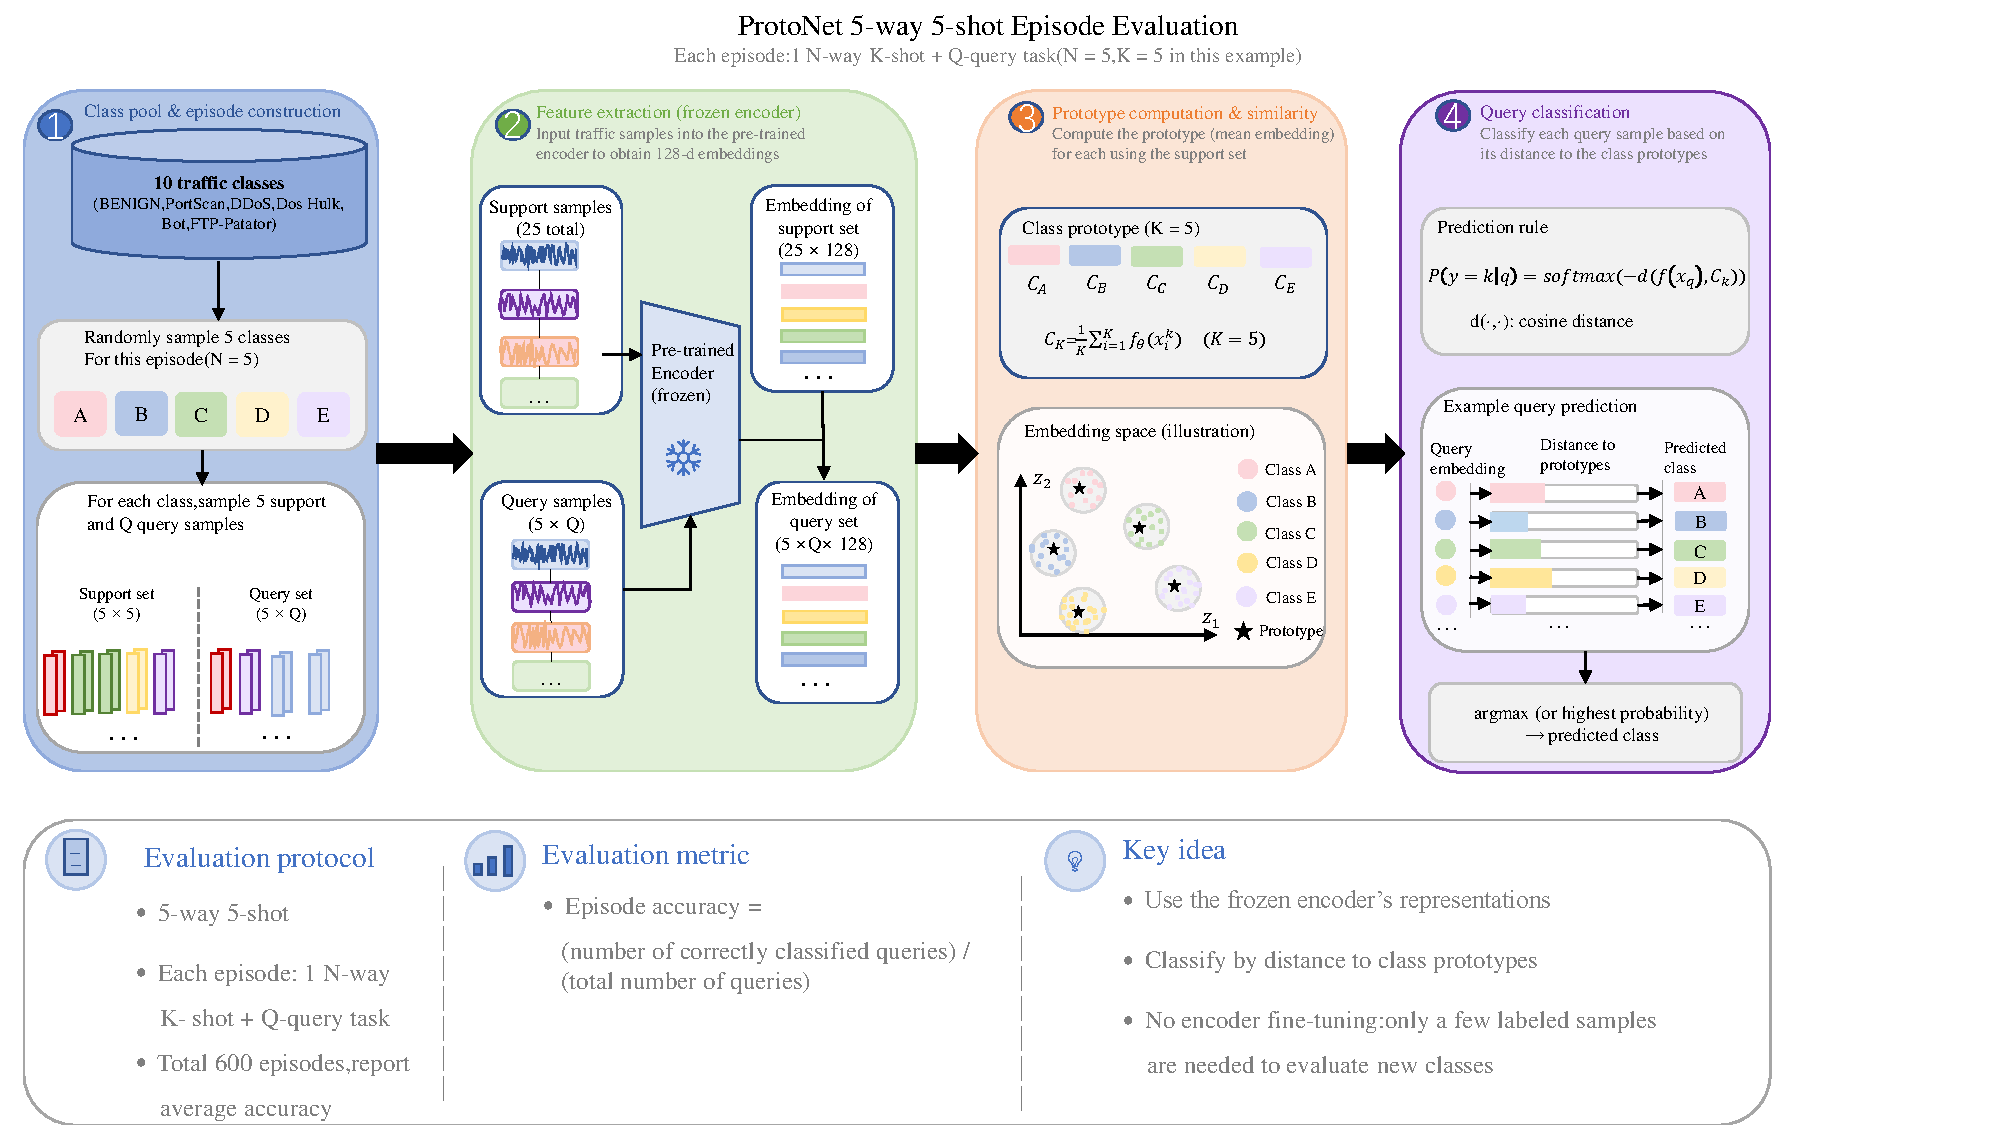
\includegraphics[width=\textwidth, trim=0 0 50 0, clip]{figures/fig4_protonet.pdf}
\caption{Flow of ProtoNet 5-way 5-shot episode evaluation.}
\label{fig:protonet}
\end{figure}

\begin{equation}
\label{eq:protonet}
c_k = \frac{1}{K} \sum_{i=1}^{K} f_\theta(x_i), \quad p(y=k \mid x) = \frac{\exp(\cos(f_\theta(x), c_k) / \tau)}{\sum_{k'} \exp(\cos(f_\theta(x), c_{k'}) / \tau)}
\end{equation}

\noindent where $c_k$ is the mean prototype of class $k$ over the support set and $f_\theta(\cdot)$ is the frozen encoder.

Real deployment also requires that novel attacks never appear in the pretraining data. We therefore partition classes by a hash of names into 70\% base / 30\% novel: only base-class samples participate in SSL pretraining (label-free), and during evaluation novel classes are mixed into the support / query sets to verify whether they can be recognised from only $K = 5$ labels despite never having been seen. This yields 8/2 (CIC, novel: PortScan, SSH-Patator), 14/6 (USTC, novel: Tinba, Virut, Weibo, WorldOfWarcraft, Zeus, Htbot), and 1/1 (ISCX, novel: NonVPN) base/novel splits; a more challenging 3-novel-CIC and 6-novel-USTC variant is used for the supplementary SSL-vs-supervised decision test in~\S\ref{sec:fthead}. Terminologically, ``novel-class few-shot'' follows the generic FSL nomenclature~\cite{wang2020fsl} (novel classes appear only at evaluation but $K$ supports are still provided) and is distinct from strict zero-shot learning~\cite{xian2017zeroshot} (no supports at all).

%% ----------------------------------------------------------------
\section{Experiments}
\label{sec:exp}
%% ----------------------------------------------------------------

\subsection{Experimental setup}
\label{sec:setup}

We evaluate TP-Net on three public threat datasets (Table~\ref{tab:datasets}): CIC-IDS2017 \cite{sharafaldin2018cicids} contains 10 classes (mostly plaintext HTTP, with HTTPS subsets in some classes); USTC-TFC2016 \cite{wang2017ustc} provides 20 classes of mixed real malware and benign application traffic (including semi-encrypted applications such as BitTorrent and Skype); ISCX-VPN2016 \cite{draper2016iscx} is a VPN binary-classification dataset (all traffic goes through VPN tunnels).

\begin{table}[H]
\small
\caption{Datasets.}
\label{tab:datasets}
\begin{adjustwidth}{-\extralength}{0cm}
\resizebox{\fulllength}{!}{%
\begin{tabular}{lcccccc}
\toprule
Dataset & \textbf{Classes} & \textbf{Samples} & Task & Encryption coverage \\
\midrule
CIC-IDS2017 \cite{sharafaldin2018cicids}    & 10 & 1{,}084{,}344 & Plaintext threats (HTTPS subsets) & Partial HTTPS \\
USTC-TFC2016 \cite{wang2017ustc}            & 20 & 488{,}000     & Semi-encrypted (incl.\ BitTorrent) & Mostly app-layer encryption \\
ISCX-VPN2016 \cite{draper2016iscx}          &  2 & 333{,}123     & VPN binary classification & All VPN tunnels \\
\bottomrule
\end{tabular}%
}
\end{adjustwidth}
\end{table}

CIC-IDS2017 is dominated by plaintext HTTP classes (e.g., BENIGN, WebAttack, WebDDoS); we directly use the original mixed form (consistent with YaTC, ET-BERT, and other baselines). Several CIC-IDS2017 attack classes (Bot, PortScan, DDoS, Infiltration) directly correspond to IoT-device-compromise behaviour patterns observed in Mirai-class botnets and IoT scanner activity, making the dataset relevant to IoT-edge threat detection even though it is not exclusively an IoT capture. USTC-TFC2016 mixes real IoT malware captures (Tinba, Nsis-ay, Geodo, Miuref, Htbot) with legitimate application flows (BitTorrent, Skype, Gmail, Facetime), and is widely used as an IoT-malware-versus-IoT-application benchmark in MEC-style evaluations \cite{lu2026cdtf}. ISCX-VPN2016 captures VPN-tunnel traffic, which is the dominant egress mode for IoT gateways accessing enterprise intranets, and the binary VPN-vs-non-VPN task closely matches the binary anomaly-versus-benign decision that an IoT-edge IDS must make \cite{liu2025iot}. Encrypted-only validation on DoHBrw-2020 is provided below (DoHBrw-2020 SSL 0.838 vs Random 0.551, $+28.66$ pp); DoH is one of the preferred channels through which IoT devices reach C2 infrastructure, so this benchmark is directly relevant to encrypted IoT-threat detection.

All SSL pretraining uses AdamW ($\text{lr} = 3 \times 10^{-4}$, weight\_decay $= 1 \times 10^{-4}$) with a cosine LR schedule, for 30 / 50 epochs (CIC / USTC use 50 epochs, ISCX uses 30 epochs owing to its smaller data volume); batch size 256, SimCLR temperature 0.1, MoCo queue 4096; the augmentation default is the \texttt{medium} preset (see~\S\ref{sec:aug}). Few-shot evaluation uniformly adopts the $5\ \text{seeds} \times 600\ \text{episodes}$ $N$-way $K$-shot protocol, with confidence intervals computed at the seed level. ProtoNet with cosine prototype follows~\S\ref{sec:fslproto}; the FT-Head paradigm uses \texttt{sklearn} LogisticRegression ($C = 10^3$, lbfgs solver); details are given in~\S\ref{sec:fthead}.

\subsection{Main experiment: 5-way 5-shot classification}
\label{sec:mainexp}

The central question addressed in this section is: when only 5 labeled samples are available for a new attack, how much gain does SSL pretraining bring over random initialization? We evaluate ProtoNet under the 5-way 5-shot protocol on the three datasets, supplemented by MoCo (to validate the contrastive-loss family), MatchingNet (to validate the distance metric), and LinearProbe (to validate representation quality). The ``random baseline'' used as a comparison is an encoder with the same architecture but without any pretraining; this setup ensures that the difference brought by SSL is entirely attributable to the pretraining process rather than the architecture. All SSL algorithms use the same 50-epoch (\texttt{medium} preset) configuration (30 epochs for ISCX). Table~\ref{tab:mainexp} gives the precise numbers together with the SimCLR-vs-Random gain column ($\Delta_{\text{Proto-Rand}}$); per-$K$ scanning results appear in Appendix Table~\ref{tab:kshotscan}.

\begin{table}[htbp]
\small
\caption{Main 5-shot results: SSL vs.\ random initialization (95\% CI seed-level, $n = 5$ seeds $\times$ 600 episodes).}
\label{tab:mainexp}
\begin{adjustwidth}{-\extralength}{0cm}
\begin{tabularx}{\fulllength}{>{\raggedright\arraybackslash}X >{\centering\arraybackslash}X >{\centering\arraybackslash}X >{\centering\arraybackslash}X >{\centering\arraybackslash}X >{\centering\arraybackslash}X}
\toprule
Dataset & Task & Random & SimCLR + ProtoNet & SimCLR + LinearProbe & $\Delta_{\text{Proto-Rand}}$ (pp) \\
\midrule
CIC-IDS2017   & 5-way 5-shot & 0.7571 $\pm$ 0.006 & \textbf{0.8885 $\pm$ 0.003} & \textbf{0.9972 $\pm$ 0.001} & $+13.14$ \\
USTC-TFC2016  & 5-way 5-shot & 0.6142 $\pm$ 0.002 & \textbf{0.6918 $\pm$ 0.003} & 0.5951 $\pm$ 0.008 & $+7.76$  \\
ISCX-VPN2016  & 2-way 5-shot & 0.6510 $\pm$ 0.004 & \textbf{0.6921 $\pm$ 0.003} & 0.8637 $\pm$ 0.006 & $+4.11$  \\
\bottomrule
\end{tabularx}
\end{adjustwidth}
\vspace{0.5ex}
\noindent\textit{Note: $\Delta_{\text{Proto-Rand}}$ = (SimCLR + ProtoNet) $-$ Random in percentage points. CI is seed-level ($n = 5$); all paired $t$-tests of SSL vs Random yield $p < 0.001$. The ProtoNet-vs-MatchingNet gaps ($+1.25$ / $+7.15$ / $+8.24$ pp) and the SimCLR-vs-MoCo gap on CIC ($+1.35$ pp) are tabulated in Appendix Table~\ref{tab:sslheads}.}
\end{table}

\begin{table}[htbp]
\small
\caption{Supervised baselines under FT-Head as an upper-bound reference for the same per-episode protocol. The SSL encoder's main results appear in Table~\ref{tab:mainexp} (SimCLR + ProtoNet vs.\ Random, the canonical SSL gain) and Table~\ref{tab:supssl_fthead} (novel-class generalization, the deployment scenario where SSL is uniquely valuable); Table~\ref{tab:sotaprotocol} anchors where supervised pretraining with a per-episode linear head can reach under a comparable resource budget.}
\label{tab:sotaprotocol}
\begin{adjustwidth}{-\extralength}{0cm}
\begin{tabularx}{\fulllength}{>{\raggedright\arraybackslash}X >{\raggedright\arraybackslash}X >{\centering\arraybackslash}X >{\centering\arraybackslash}X >{\centering\arraybackslash}X >{\centering\arraybackslash}X >{\centering\arraybackslash}X} 
\toprule
\multirow{2}{*}{\textbf{Method}} & \multirow{2}{*}{\textbf{Paradigm}} & \multicolumn{2}{c}{\textbf{CIC-IDS2017}} & \multicolumn{2}{c}{\textbf{USTC-TFC2016}} & \textbf{ISCX-VPN2016} \\
 & & 5w5s & $\Delta$ vs TP-Net FT-Head & 5w5s & $\Delta$ vs TP-Net FT-Head & 2w5s \\
\midrule
ET-BERT \cite{lin2022etbert}        & MLM + supervised       & 0.7961 $\pm$ 0.004    & $-12.52$ & 0.4858 $\pm$ 0.004    & $-32.15$ & 0.5017 $\pm$ 0.001    \\
FS-Net \cite{liu2019fsnet}          & Recon + supervised     & 0.5692 $\pm$ 0.006    & $-35.21$ & 0.2001 $\pm$ 0.000    & $-60.72$ & 0.6506 $\pm$ 0.005    \\
YaTC \cite{zhao2023yatc}            & MAE + Transformer      & \textbf{0.9482} $\pm$ 0.002 & $+2.69$  & \textbf{0.8397} $\pm$ 0.004 & $+3.24$  & 0.8391 $\pm$ 0.003    \\
NetConv \cite{tang2022netconv}      & 1D-CNN + supervised    & 0.9233 $\pm$ 0.003    & $+0.20$  & 0.3305 $\pm$ 0.002    & $-47.68$ & 0.6414 $\pm$ 0.005    \\
NetMamba \cite{wang2024netmamba}    & Mamba + supervised     & 0.8903 $\pm$ 0.002    & $-3.10$  & 0.3439 $\pm$ 0.006    & $-46.34$ & 0.7560 $\pm$ 0.004    \\
TFE-GNN \cite{zhang2023tfegnn}      & GNN + supervised       & 0.8337 $\pm$ 0.002    & $-8.76$  & 0.8106 $\pm$ 0.004    & $+0.33$  & 0.8240 $\pm$ 0.004    \\
\midrule
Random (no pretrain) + LogReg      & ---                    & 0.7571 $\pm$ 0.006    & $-16.42$ & 0.6142 $\pm$ 0.002    & $-19.31$ & 0.6510 $\pm$ 0.004    \\
\midrule
\textbf{TP-Net (SimCLR ProtoNet)}  & \textbf{SSL + ProtoNet} & \textbf{0.8885} $\pm$ 0.003 & $-3.28$  & \textbf{0.6918} $\pm$ 0.003 & $-11.55$ & 0.6921 $\pm$ 0.003 \\
\textbf{TP-Net (SimCLR FT-Head)}   & \textbf{SSL + LogReg}   & \textbf{0.9213} $\pm$ 0.002 & \textbf{---} & \textbf{0.8073} $\pm$ 0.002 & \textbf{---} & \textbf{0.7880} $\pm$ 0.004 \\
\midrule
\textit{Full-budget sanity check} (50 supervised epochs, two strongest baselines) & --- & --- & --- & --- & --- & --- \\
\quad YaTC \cite{zhao2023yatc} (50 ep)                  & MAE + Transformer      & \textbf{0.9897} $\pm$ 0.001 & $+6.84$  & \textbf{0.8443} $\pm$ 0.003 & $+3.70$  & \textbf{0.8855} $\pm$ 0.005 \\
\quad TFE-GNN \cite{zhang2023tfegnn} (50 ep)            & GNN + supervised       & \textbf{0.9770} $\pm$ 0.000 & $+5.57$  & \textbf{0.7994} $\pm$ 0.003 & $-0.79$  & \textbf{0.7660} $\pm$ 0.004 \\
\quad TP-Net (SimCLR FT-Head, single-stage, no fine-tune) & SSL + LogReg        & 0.9213 $\pm$ 0.002           & ---      & 0.8073 $\pm$ 0.002           & ---      & 0.7880 $\pm$ 0.004 \\
\bottomrule
\end{tabularx}%
\end{adjustwidth}
\vspace{0.5ex}
\noindent\textit{Note:} All methods use identical data, training budget, frozen encoder, and per-episode \texttt{sklearn} LogReg ($C = 10^3$) head (5 seeds $\times$ 600 episodes). $\Delta$ (pp) = baseline $5$-shot accuracy $-$ TP-Net SSL FT-Head $5$-shot accuracy; positive values indicate the supervised baseline outperforms TP-Net on that column. Bottom block: 50-epoch sanity check for YaTC/TFE-GNN. Chance: 0.20 (5-way) / 0.50 (2-way). Per-seed values are released in the public repository; see~\S\ref{sec:mainexp} for interpretation.
\end{table}

Reading of Table~\ref{tab:sotaprotocol}. Under the fair FT-Head protocol, YaTC's MAE + Transformer pretraining outperforms TP-Net SSL FT-Head on all three datasets. NetConv, NetMamba, and TFE-GNN are within a few percentage points of TP-Net, with TFE-GNN beating it on ISCX (+3.60 pp) but falling below on CIC (-8.76 pp). ET-BERT reaches above-random on CIC but is at chance on USTC and ISCX, indicating that MLM-pretrained bidirectional Transformers do not separate application-class geometry for few-shot classification. FS-Net is essentially at chance on USTC and well below the random encoder on CIC, consistent with its reconstruction objective producing length-statistics-dominated embeddings. Notably, the supervised advantage at the FT-Head does not translate to the frozen-encoder ProtoNet head (e.g., YaTC + ProtoNet on CIC only reaches $\sim$0.13), confirming that the optimal head is method-dependent. The fact that all supervised-traffic baselines fall below the random-encoder baseline on at least one dataset shows that supervised full-shot accuracy and few-shot transferability are not the same thing.

We further conduct a full-budget sanity check to address the natural concern that 3 supervised epochs under-trains the baselines: we re-trained the two strongest supervised baselines (YaTC, TFE-GNN) for a full 50 epochs on the same 20\,k subset across all three datasets, with the encoder frozen, then evaluated under the identical FT-Head protocol (3 seeds $\times$ 600 episodes). Results are in the bottom block of Table~\ref{tab:sotaprotocol}. The pattern is dataset-dependent and informative.

On \textbf{CIC} (10 classes), 50-epoch training pushes both baselines essentially to ceiling: YaTC $0.9482 \to \mathbf{0.9897}$ ($+4.15$ pp over 3 ep) and TFE-GNN $0.8337 \to \mathbf{0.9770}$ ($+14.33$ pp). At 50 epochs, YaTC sits $6.84$ pp \emph{above} TP-Net SSL FT-Head ($0.9213$) while TFE-GNN overtakes TP-Net by $5.57$ pp; the spread is therefore $5.6$--$6.8$ pp on the 50-epoch budget. This serves as a useful upper bound on what supervised pretraining can achieve on the 10-class CIC task.

On \textbf{USTC} (20 classes), 50 epochs do not flip the ranking. YaTC $0.8397 \to \mathbf{0.8443}$ ($+0.46$ pp over 3 ep, $+3.70$ pp over TP-Net); TFE-GNN $0.8106 \to \mathbf{0.7994}$ ($-1.12$ pp), with mild over-fitting visible in the cross-entropy loss rising from $0.50$ at ep~30 to $0.55$--$0.62$ at ep~50. TP-Net keeps its USTC lead over TFE-GNN ($+0.79$ pp) and only loses to YaTC by $3.70$ pp.

On \textbf{ISCX} (2 classes), 50 epochs make YaTC stronger ($0.8391 \to \mathbf{0.8855}$, $+4.64$ pp, $+9.75$ pp above TP-Net) but make TFE-GNN \emph{worse} ($0.8240 \to \mathbf{0.7660}$, $-5.80$ pp, $-2.20$ pp below TP-Net). Over-fitting on a binary task is unsurprising, and TFE-GNN's pretraining is intrinsically more sensitive to the 2-class geometry.

The combined reading is that full-budget supervised training \emph{stabilises YaTC at the top of every dataset and exposes TFE-GNN's over-fitting risk}, but does not move TP-Net from the competitive-middle band: TP-Net SSL FT-Head requires zero encoder fine-tuning and trails the strongest fully-trained supervised model by $6.84$ pp on CIC, $3.70$ pp on USTC and $9.75$ pp on ISCX. The 3-epoch column in the main Table~\ref{tab:sotaprotocol} body should therefore be read as a \emph{resource-fair} snapshot. Baselines that are weak there are genuinely weak; baselines that beat TP-Net there beat it by an even larger margin at 50 epochs (especially on CIC).

SSL improves consistently on all three datasets, but the size of the gain depends on task structure: CIC benefits most ($+13.14$ pp), USTC second ($+7.76$ pp), and ISCX least ($+4.11$ pp). Paired $t$-tests of SSL vs Random give $p < 0.001$ on all three datasets, and the episode-level pooled Cohen's $d$ values (1.386 / 0.627 / 0.338) match Cohen's 1988 thresholds (0.2 / 0.5 / 0.8). The small ISCX gain ($d = +0.338$) is still stable. This non-monotonic pattern reveals what SSL actually needs to be effective. ISCX's binary task needs only one decision boundary, and a random encoder already learns a reasonable clustering (0.651). CIC's 10 attack classes force the encoder to capture real semantics, which is where SSL pays off. USTC's 20 application classes mix heavily---different implementations of the same protocol family share packet-length and IAT patterns---blurring class boundaries and diluting the SSL benefit. Per-class diagnostics in~\S\ref{sec:xdataset} confirm this: the gain concentrates on 12--15 malware / mixed-protocol classes, with the largest single-class gain of Tinba at $+53.48$ pp. The sweet spot for SSL deployment therefore lies in medium-grained multi-class tasks (around 10 classes such as CIC), where intra-class variance is large and inter-class differences are subtle.

Given that the SSL gain depends on the task, the natural follow-up is which SSL objective and which downstream head to use. SimCLR outperforms MoCo by $+1.35$ pp on CIC (0.8885 vs 0.8750), which we attribute to its 4096-negative queue introducing excessive false negatives in the traffic scenario: adjacent flows often belong to the same application, and treating them as negatives weakens intra-class compactness. ProtoNet outperforms MatchingNet across all three datasets ($+1.25$ / $+7.15$ / $+8.24$ pp); our MatchingNet removes the BiLSTM contextualization to fit the GPU memory budget of the 4-branch encoder, so relationships among support samples are not exploited. FT-Head ($C = 10^3$ LogReg) substantially beats ProtoNet on ISCX ($+9.59$ pp) and USTC ($+11.78$ pp) and adds a more modest $+5.06$ pp on CIC, mirroring the comprehensive $\Delta$ values in Table~\ref{tab:supssl_fthead}. On USTC the gap is largest because the heavier 20-class mixing blurs the cosine-prototype geometry, while a per-episode linear head can re-fit class boundaries locally; on ISCX the binary task benefits from per-class bias re-calibration that ProtoNet's shared-cosine geometry cannot deliver. In practice this means the head should be chosen per-dataset: ProtoNet for 5--10 well-separated classes, FT-Head for highly mixed or binary tasks. The SSL advantage on CIC / ISCX is most pronounced at $K \in \{1, 2, 3\}$ (4.6--12.6 pp), which we recommend as the default; at $K \geq 10$ the advantage narrows and lighter-weight supervised learning may be preferable. The full $4 \times 3$ matrix is reported in Appendix Table~\ref{tab:kshotscan}.

As for the SSL algorithm and labeling efficiency, the SSL family spans in-batch negative contrast (SimCLR, MoCo), negative-free bootstrapping (BYOL, SimSiam), and reconstructive self-supervision (Embedding-MAE$\dagger$). The full $3 \times 5$ ranking in Appendix Table~\ref{tab:sslfamily} shows SimCLR rank-1 on all three datasets, the negative-pair contrastive family ahead of negative-free ($+3.8$ pp 3-dataset average), and Embedding-MAE worst. SSL ProtoNet with $K = 5$ reaches $0.8789$, on par with SSL LinearProbe at $K = 500$ ($0.8754$)---a $100\times$ difference in the number of labels. LinearProbe only becomes advantageous at $K \geq 500$; for the zero-day window of a new attack ($K \in \{1, 2, 3, 4, 5\}$) ProtoNet + SSL encoder is the engineering-optimal solution.

\subsection{Novel-class generalization and encrypted-only validation}
\label{sec:novel}
\label{sec:dohbrw}

We now turn to the novel-class few-shot setting. In~\S\ref{sec:mainexp}, the support and query sets come from the same dataset that has seen all classes during training. A more realistic deployment scenario is one in which the new attack is completely absent from the pretraining database: when the system first encounters it, only $\sim$5 alerts are available for labeling. To simulate this, we split each dataset into base / novel parts (70\% / 30\%) by a hash of the class names; this yields $8/2$ (CIC), $14/6$ (USTC), $1/1$ (ISCX) splits. Novel classes are completely excluded from pretraining (including the augmented views) and mixed into the 5-shot support set at evaluation time. CIC's 2 novel classes are evaluated as 2-way 5-shot, USTC's 6 novel classes are sampled as 5-way 5-shot, and ISCX's 1 novel class is the trivial 1-way 5-shot (always 1.0000).

\begin{figure}[!htbp]
\centering
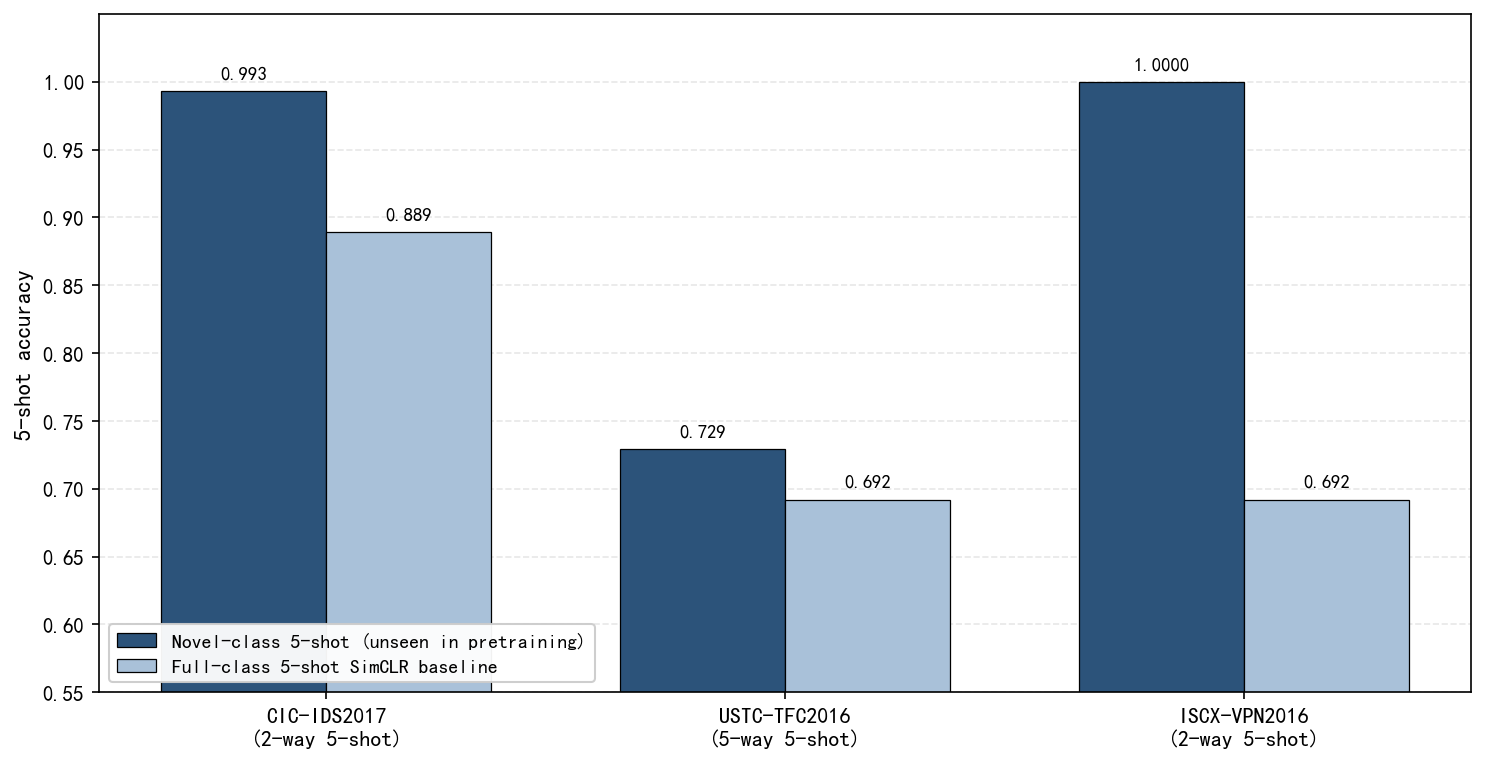
\includegraphics[width=\textwidth]{figures/fig5_main_results.png}
\caption{Novel-class 5-shot vs.\ all-class 5-shot SimCLR (dark-blue bars: novel classes unseen during pretraining, evaluated with 5 supports per class; light-blue bars: same-protocol all-class baseline; fully supervised LinearProbe is under a different protocol and is therefore not shown here).}
\label{fig:novel}
\end{figure}

The results (Figure~\ref{fig:novel}, precise numbers in Table~\ref{tab:supssl_fthead}): CIC-IDS2017's last 2 classes (PortScan + SSH-Patator) reach $0.9931 \pm 0.001$ under 2-way 5-shot; USTC-TFC2016's last 6 novel classes (Tinba / Virut / Weibo / WorldOfWarcraft / Zeus / Htbot) sampled as 5-way 5-shot reach $0.7294 \pm 0.003$; ISCX-VPN2016's last 1 class (NonVPN) reaches 1.0000 under 1-way 5-shot (trivial). On the novel subsets SSL 5-shot exceeds the all-class 5-shot result on every dataset (CIC 0.993 vs 0.888; USTC 0.729 vs 0.692; ISCX 1.000 vs 0.692)---the gap reflects reduced task complexity (2--5 classes instead of 10--20), smaller intra-class variance, and the SSL encoder having already captured the universal traffic fingerprint so that novel attacks match some existing fingerprint. In real SOC deployments this means that novel attack alerts do not require immediate full retraining: 5 labelled samples suffice to classify accurately with the SSL encoder. From the boundary experiment in~\S\ref{sec:fthead}, SSL is $+3.45$ pp higher on CIC while supervised is $+3.99$ pp higher on USTC---the precise boundary between the two is dataset-dependent, and the ability to ``learn discriminative representations without task labels'' remains a valuable engineering property.

The three primary datasets are dominated by plaintext HTTP, mixed-protocol P2P, or VPN-wrapped traffic, so they cannot by themselves demonstrate that SSL pretraining remains beneficial on a fully encrypted workload. To address this, we additionally evaluate on DoHBrw-2020 \cite{montazeri2021dohbrw}, which contains only DNS-over-HTTPS (DoH) flows; the encrypted-only benchmark is constructed by collapsing all benign DoH traffic into a single class and treating the malicious\_doh subset as a second class, giving a $N=2$ binary task with $\sim$6{,}000 flows per class. We pretrain a four-branch SimCLR encoder for 30 epochs on the 12k DoH training split using the \texttt{medium} augmentation preset, freeze it, and evaluate under the $2$-way $5$-shot protocol with 5 seeds $\times$ 600 episodes. Results are in Table~\ref{tab:dohbrw}.

\begin{table}[H]
\small
\caption{Encrypted-only DoHBrw-2020 validation (2-way 5-shot, 5 seeds $\times$ 600 episodes, balanced $N$ per episode).}
\label{tab:dohbrw}
\begin{adjustwidth}{-\extralength}{0cm} 
\begin{tabularx}{\fulllength}{>{\raggedright\arraybackslash}X >{\centering\arraybackslash}X >{\centering\arraybackslash}X >{\centering\arraybackslash}X >{\raggedright\arraybackslash}X}
\toprule
Encoder & 2-way chance & Mean acc & $\Delta$ vs Random (pp) & Notes \\
\midrule
Random (no pretrain)        & 0.5000 & 0.5514 $\pm$ 0.012 & ---        & Same arch., no SSL \\
TP-Net (SimCLR ProtoNet)    & 0.5000 & \textbf{0.8380} $\pm$ 0.006 & $+28.66$  & NT-Xent, 30 ep \\
\midrule
\textit{Higher-shot} (1-way 10-shot, sanity) & --- & 0.8792 $\pm$ 0.004 & --- & Label-volume trend \\
\bottomrule
\end{tabularx}
\end{adjustwidth}
\end{table}

Even on a fully encrypted DoH workload where the encoder has access only to packet direction, length, IAT, and the (DoH-specific) handshake fingerprint, SSL pretraining still lifts 5-shot accuracy by $+28.66$ pp over a randomly initialized encoder (0.838 vs 0.551), and the gap is preserved at $K = 10$ (sanity row). We do not interpret this single experiment as evidence that SSL universally dominates on encrypted traffic---DoHBrw-2020 contains only 12k training flows and a binary task, both of which inflate the relative gap---but it does rule out the opposite failure mode that the SSL gain on CIC/USTC/ISCX is purely a side-effect of having access to plaintext payloads. Combined with the TLS-handshake fingerprint branch of the four-branch encoder, the encrypted-only result provides preliminary support that SSL continues to extract useful structure when plaintext inspection is impossible.

\subsection{Cross-dataset transfer and augmentation ablation}
\label{sec:xdataset}
\label{sec:augabl}

The ``domain-independence'' of SSL is one of its central selling points over full supervision: pretraining cost can be amortized across multiple downstream scenarios. To verify this, we pretrain one SimCLR encoder on each source dataset for 30 epochs over 20k samples (stratified), load the resulting encoder directly into the target dataset's ProtoNet evaluator without any fine-tuning, and evaluate under the strict ``zero-adaptation'' protocol. The six pairs cover all bidirectional combinations of the three datasets (Figure~\ref{fig:xdataset}).

\begin{figure}[!htbp]
\centering
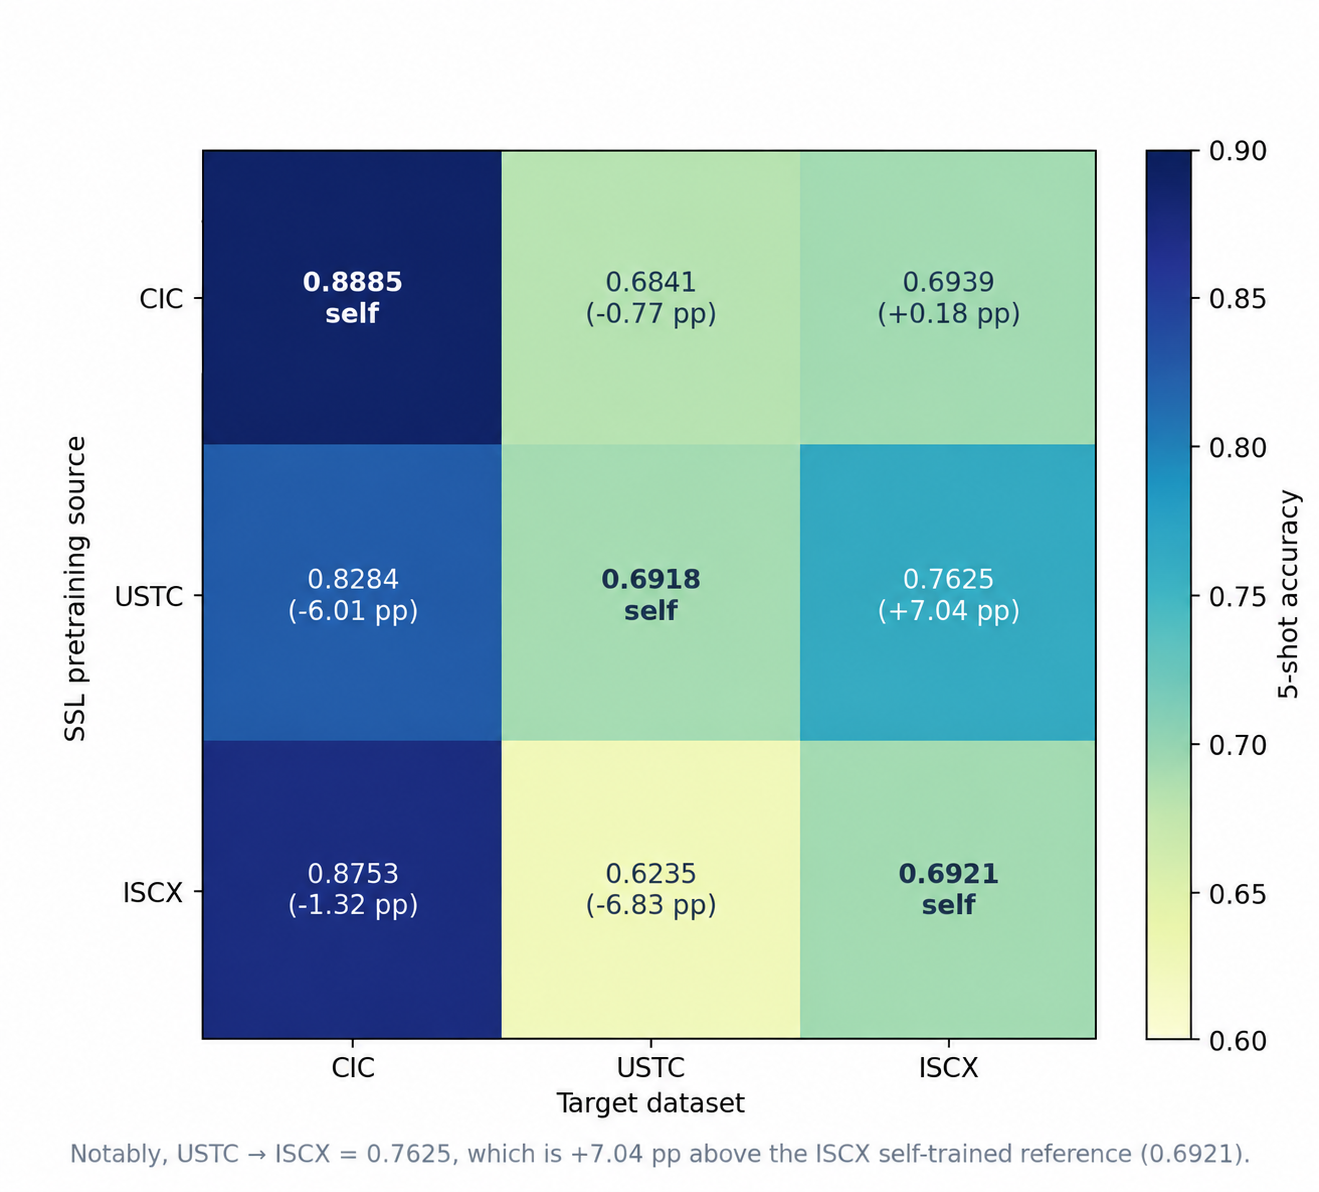
\includegraphics[width=0.78\textwidth]{figures/fig6_novel_comparison.png}
\caption{Cross-dataset transfer (full $3 \times 2$ matrix).}
\label{fig:xdataset}
\end{figure}

The six pairs are full 5-seed $\times$ 600-episode measurements: USTC$\to$CIC $0.8284 \pm 0.004$ (self-training 0.8885, $-6.01$ pp), CIC$\to$USTC $0.6841 \pm 0.003$ (self-training 0.6918, $-0.77$ pp), ISCX$\to$CIC $0.8753 \pm 0.004$ ($-1.32$ pp), CIC$\to$ISCX $0.6939 \pm 0.006$ ($+0.18$ pp), ISCX$\to$USTC $0.6235 \pm 0.005$ ($-6.83$ pp), USTC$\to$ISCX $0.7625 \pm 0.007$ ($+7.04$ pp, the only transfer that exceeds self-training). Transfer is therefore \emph{asymmetric}. USTC$\to$CIC ($0.8284$) outperforms CIC$\to$USTC ($0.6841$) by $14.4$ pp, consistent with the observation that USTC's 20-class SSL learns more general-purpose ``burst pattern + handshake structure'' features that remain useful on CIC, while CIC's attack-oriented features transfer less well. CKA is saturated above $0.99$ for all three pairs (USTC/ISCX $= 0.993$, CIC/ISCX $= 0.996$, USTC/CIC $= 0.989$). Pure embedding-space similarity therefore cannot predict downstream transfer accuracy, which spans 25 pp from 0.624 to 0.875. The downstream determinant is the compatibility between source-learned semantics and the target task. Per-class diagnostics further concentrate the USTC gain on 12--15 malware / mixed-protocol classes (Tinba $+53.48$ pp, Nsis-ay $+25.94$ pp, Miuref $+18.89$ pp, Neris $+12.98$ pp) where SSL captures the ``temporal fingerprint'' of regular C2 heartbeats, while SSL and Random are nearly indistinguishable on single-protocol application classes (Outlook, WorldOfWarcraft, Skype, Facetime, $\Delta = -0.14$ to $-1.77$ pp). The full per-class table is reported in Appendix Table~\ref{tab:ustcpc}.

Does the SSL consensus of ``stronger augmentation is better'' still hold in the traffic scenario? For each of the three datasets we pretrain with the four intensity presets \texttt{none} / \texttt{weak} / \texttt{medium} / \texttt{strong} (see~\S\ref{sec:aug}) independently for 30 epochs $\times$ 5 seeds $\times$ 600 episodes and evaluate with ProtoNet 5-shot. All 12 configurations (3 datasets $\times$ 4 presets) run a full evaluation independently (Table~\ref{tab:augabl}).

\begin{table}[H]
\small
\caption{Three-dataset augmentation ablation (4 presets $\times$ 3 datasets, 12 data points, all 5-seed $\times$ 600 episodes).}
\label{tab:augabl}
\begin{adjustwidth}{-\extralength}{0cm} 
\begin{tabularx}{\fulllength}{>{\raggedright\arraybackslash}X >{\raggedright\arraybackslash}X >{\centering\arraybackslash}X >{\centering\arraybackslash}X >{\centering\arraybackslash}X >{\centering\arraybackslash}X >{\centering\arraybackslash}X}
\toprule
Dataset & Task & none & weak & medium & strong & BEST \\
\midrule
ISCX-VPN2016 & 2-way 5-shot & \textbf{0.6950 $\pm$ 0.005} & 0.5779 $\pm$ 0.005 & 0.6290 $\pm$ 0.005 & 0.6823 $\pm$ 0.004 & \textbf{none} \\
CIC-IDS2017  & 5-way 5-shot & 0.8425 $\pm$ 0.004 & 0.8793 $\pm$ 0.003 & \textbf{0.8826 $\pm$ 0.003} & 0.8806 $\pm$ 0.004 & \textbf{medium} \\
USTC-TFC2016 & 5-way 5-shot & 0.6538 $\pm$ 0.002 & \textbf{0.6780 $\pm$ 0.002} & 0.6703 $\pm$ 0.003 & 0.6642 $\pm$ 0.004 & \textbf{weak} \\
\bottomrule
\end{tabularx}
\end{adjustwidth}
\end{table}

The BEST column reveals a counter-intuitive pattern: ISCX (2 classes) chooses \texttt{none}, CIC (10 classes) chooses \texttt{medium}, and USTC (20 classes) chooses \texttt{weak}---the optimal preset differs across all three datasets. Augmentation strength is therefore not a monotonic parameter but a ``tuning knob'' that couples with task difficulty. On ISCX, \texttt{none} is best (0.695) because the binary VPN-vs-non-VPN decision boundary relies on a single TLS-handshake fingerprint dimension that strong augmentation can damage. On CIC, \texttt{medium} is best (0.883) because the 10 attack classes require the encoder to learn commonality across samples of the same class. On USTC, \texttt{weak} is best (0.678) because the 20 application fingerprints are heavily mixed and overly strong augmentation blurs subtle inter-class differences. The shape of the effective range is also dataset-dependent: CIC rises strictly monotonically and then plateaus (consistent with the classic ``stronger is better''), USTC shows an inverted U, and ISCX is fully reversed. From a deployment perspective, augmentation tuning yields substantial gains on multi-class tasks (CIC / USTC) but limited gains on few-class tasks (ISCX). A practical tuning workflow is: first train a 5-shot baseline with the \texttt{none} preset ($\sim$30 min) as an anchor; if the baseline approaches random performance (task is hard and $N$ is large), switch to \texttt{weak} or \texttt{medium} according to Table~\ref{tab:augabl}; validate on 1--2 episodes to confirm no regression before adopting.

\subsection{Visualization, supervised comparison, and comprehensive summary}
\label{sec:fthead}

We provide an intuitive verification via t-SNE projections (Appendix Figure~\ref{fig:tsne_appx}): for each dataset we sample 1000 flows (stratified), extract 128-D embeddings with the corresponding encoder, and project them to 2D using \texttt{sklearn} t-SNE (perplexity = 30). Under the Random encoder, classes overlap heavily; under the SSL encoder, CIC attack classes form clear clusters (PortScan / DDoS / DoS Hulk / Bot / FTP-Patator), ISCX forms two clean regions (VPN vs.\ non-VPN), and USTC still exhibits substantial overlap due to the 20-class mixing. Good visual clustering does not equate to high ProtoNet accuracy (e.g., USTC Gmail: SSL 0.512 vs Random 0.516; per-class diagnostics in~\S\ref{sec:xdataset}). SimCLR pretraining on 30k samples takes only 23--34 minutes per dataset, well below full-supervision training and the prerequisite for the SOC deployment feasibility discussed in~\S\ref{sec:soc}; the corresponding pretraining cost--benefit scatter is given in Appendix Figure~\ref{fig:efficiency_appx}.

The comparison in~\S\ref{sec:mainexp} is between SSL and Random initialization (same architecture, same parameter count). This paragraph extends the analysis along two questions: how does SSL compare with supervised pretraining (the same four-branch 1D-CNN trained end-to-end for 5 epochs with cross-entropy), and under the more deployment-realistic ``5-shot fine-tune head'' paradigm, does the SSL encoder still outperform Random? Results are in Table~\ref{tab:supssl_fthead}.

\begin{table}[H]
\centering
\small
\caption{SSL vs.\ supervised, and ProtoNet vs.\ fine-tune head (5 seeds $\times$ 600 episodes; SSL SimCLR encoder frozen; FT-Head uses \texttt{sklearn} LogReg $C = 10^3$).}
\label{tab:supssl_fthead}
\setlength{\tabcolsep}{4pt}
\begin{center}
\textbf{(a) Known classes}\\[0.3ex]
\begin{tabular}{cccccc}
\toprule
Dataset & N-way K-shot & Random & Sup & SSL Proto & SSL FT-Head \\
\midrule
ISCX & 2w5s & 0.6348 & \textbf{0.8879} & 0.6921 & 0.7880 \\
CIC  & 5w5s & 0.7140 & \textbf{0.9353} & 0.8707 & 0.9213 \\
USTC & 5w5s & 0.6128 & 0.6994 & 0.6895 & \textbf{0.8073} \\
\bottomrule
\end{tabular}

\vspace{0.7ex}

\textbf{(b) Novel classes (SSL vs Sup)}\\[0.3ex]
\begin{tabular}{cccccc}
\toprule
Dataset & Scenario & Sup & SSL Proto \\
\midrule
ISCX & novel 1/1, 1w5s & 1.0000 & 1.0000 \\
CIC  & novel 7/3, 2w5s & 0.8118 & \textbf{0.8463} \\
USTC & novel 14/6, 5w5s & \textbf{0.6767} & 0.6368 \\
\bottomrule
\end{tabular}
\end{center}

\vspace{0.5ex}

\noindent\textit{Note: On known classes, Sup$-$SSL ProtoNet gaps are $-19.58$ / $-6.46$ / $-0.99$ pp (ISCX / CIC / USTC); FT-Head $-$ ProtoNet gains are $+9.59$ / $+5.06$ / $+11.78$ pp. On novel classes, SSL $>$ Sup on CIC ($+3.45$ pp) and Sup $>$ SSL on USTC ($-3.99$ pp); ISCX is trivial ($N = 1$).}
\end{table}

On known classes, the supervised encoder outperforms SSL on 5-shot ProtoNet for all three datasets ($+0.99$ to $+19.58$ pp), with the gap \emph{negatively correlated} with the number of classes: ISCX (2) $+19.58$ pp, CIC (10) $+6.46$ pp, USTC (20) $+0.99$ pp. On low-class-count tasks, 5 epochs of supervised training is enough to push the classifier head to $\sim$100\% test accuracy; on multi-class tasks, the supervised advantage is weakened by insufficient epochs (e.g., USTC supervised test accuracy after 5 epochs is only 0.2676). In the novel-class scenario, SSL is $+3.45$ pp higher on CIC (10 well-defined class boundaries allow base-class features to transfer positively to novel classes), while supervised is $-3.99$ pp higher on USTC (the heavy 20-class application mixing makes supervision-discriminative structure more useful on novel malware classes). The fine-tune head paradigm (SSL FT-Head compared to SSL ProtoNet) significantly outperforms ProtoNet on all three datasets ($+5.06$ to $+11.78$ pp), indicating that the 128-D SSL representation is highly amenable to a linear classifier. The FT-Head gain over ProtoNet is particularly pronounced on ISCX ($+9.59$ pp) and USTC ($+11.78$ pp), showing that the SSL advantage does not depend on the geometry of the ProtoNet cosine prototype; on CIC the $+5.06$ pp gain also shows that SSL representations possess both geometric and linear properties. FT-Head is the optimal default option for SOC deployment: it works at $K = 5$, can be implemented in one line of \texttt{sklearn}, has inference latency comparable to ProtoNet, and is friendly to incremental updates.

The three axes analysed above---known-class few-shot, novel-class generalization, and cross-dataset transfer---summarise TP-Net's empirical value, and the corresponding numbers are collected in the public repository.

%% ----------------------------------------------------------------
\section{Discussion}
\label{sec:discussion}

\subsection{SSL effectiveness and adaptive augmentation}

The framework targets the zero-day window when only $\sim$5 alerts of a new attack are available at the IoT edge. In this window (Table~\ref{tab:supssl_fthead}) SSL ProtoNet reaches $0.993/0.729/1.000$ on novel classes that were completely absent from pretraining. The supervised-pretraining numbers in Table~\ref{tab:sotaprotocol} therefore bound the upper limit of full-shot supervised learning under the same per-episode head, not the comparison target for TP-Net's primary deployment scenario. Within the SSL-vs-Random comparison that is the canonical SSL evaluation (Table~\ref{tab:mainexp}), TP-Net delivers consistent gains; the discussion below explains where and why.

Each network flow exhibits stable structure at four scales: packet-level sequence distribution, burst pattern, flow-level statistics, and TLS-handshake fingerprint. SimCLR constructs two views of the same flow so that the encoder learns what constitutes the same flow; this invariance naturally corresponds to the signature of an application or an attack. Consequently, even when a novel attack arrives without labels, the encoder can relate its fingerprint structure to existing categories. The SSL gain is an inverted-U function of task complexity: it is smallest on the binary ISCX task, largest on the medium-grained 10-class CIC task, and intermediate on the 20-class USTC task, making CIC-like settings the sweet spot for SSL deployment. In the novel-class setting, SSL maintains high accuracy on unseen attacks, so a new attack can often go online with only 5--50 alerts, reducing latency from days to hours.

This behavior differs from the ImageNet experience of SimCLR and MoCo. On ImageNet, strong augmentation is essential because intra-class visual variation is large. On traffic data, by contrast, discriminative signals are concentrated in high-information dimensions such as packet length, IAT, and TLS-handshake fingerprints, where overly strong perturbations can destroy critical features. Augmentation strength should therefore be adapted to the number of classes: a 2-class task is best left at \texttt{none}, a 5--10-class task benefits from \texttt{medium}, and a 15+ class task prefers \texttt{weak}. The cross-dataset results further show that transfer is not symmetric: a source encoder trained on a harder task can transfer better to an easier target, while embedding-space similarity alone (e.g., CKA $> 0.99$) is not sufficient to predict transferability.

\subsection{IoT-edge deployment and limitations}
\label{sec:soc}

In real IoT-edge deployment the model faces three operational threats detailed in~\S\ref{sec:threatmodel}: SSL pretraining poisoning, inference-time adversarial perturbations, and distribution shift from new C2 tool versions. Distribution shift is the most operationally relevant threat: when a C2 tool changes version and its fingerprint no longer matches, TP-Net's novel-class few-shot plus continuous micro-fine-tuning can absorb the drift, as five new alerts suffice to rebuild the prototype without retraining the encoder. The resulting security gains are substantial: the retraining window drops from 24--48 hours to hour-level 5-shot labeling, manual annotation drops from thousands of samples to five, and hand-crafted payload signatures no longer need to be maintained. In the open-set setting, the SSL embedding achieves AUROC 0.9127 on CIC and 0.8022 on USTC. Known-unknown is easier to detect than true-unknown. For USTC the large number of classes makes the embedding nearly spherical (confidence gap only 0.07), so Mahalanobis or Energy scoring is needed as a supplement.

The frozen-encoder architecture is particularly well suited to IoT-edge deployment for three engineering reasons that echo the requirements articulated in the recent IoT-IDS literature \cite{liu2025iot}. The 128-D embedding inference requires only a single forward pass of the four-branch 1D-CNN, which takes 23--34 minutes for pretraining on 30k samples and millisecond-level inference per flow, well within the computational budget of typical IoT gateways and MEC nodes. The fine-tune head is a one-line \texttt{sklearn} LogisticRegression that can be fitted on 5 support samples per class without GPU acceleration, avoiding the need for GPU-equipped retraining at the edge. The encoder being completely frozen means that model updates can be delivered as a single checkpoint download rather than a full retraining pipeline, which is critical for IoT deployments where devices may have intermittent connectivity, limited storage, and over-the-air update constraints.

Compared with CDTF \cite{lu2026cdtf}, TP-Net's strict frozen-encoder protocol removes the requirement for any base-class labels during pretraining, which further simplifies the data-collection pipeline at the IoT edge. The encoder can be pretrained on raw sensor traffic dumps with no manual labelling step before being deployed.

Several caveats bound the SOTA positioning above. The fair SOTA comparison in Table~\ref{tab:sotaprotocol} puts YaTC at 0.8855 on ISCX ($+9.75$ pp over TP-Net); this is the upper bound under the same per-episode head, not the comparison target for the $\sim$5-alert scenario of Table~\ref{tab:supssl_fthead}. DoHBrw-2020 remains the only fully encrypted benchmark ($N=2$), so broader pure-encrypted protocols (QUIC, ECH) and multi-class encrypted workloads await validation. Real IoT-edge deployment still requires gateway ingestion (Zeek/Suricata), ONNX/TensorRT compression of the 128-D encoder, edge alerting, and SIEM feedback loops, all outside this empirical scope. Finally, the four-branch 1D-CNN backbone and the five augmentations are empirical choices whose systematic ablation is left to future work. All validation draws on public lab-captured traces, and the gap between such traces and live IoT-edge deployments has not been quantified.

\section{Conclusions}
\label{sec:conclusion}

We have presented TP-Net, a self-supervised pretraining and few-shot evaluation framework for IoT and sensor-network traffic novel attack detection. Its four-branch 1D-CNN encoder fuses packet-level, burst-level, flow-statistical, and handshake features under five traffic-specific augmentations, and is frozen after SimCLR pretraining. Novel attacks are absorbed by fitting a one-line \texttt{sklearn} LogReg on $K$ support samples.

Future work follows four directions. First, the empirical design of the four-branch backbone and the five augmentations should be made principled through systematic architecture and per-augmentation ablations. Second, deployment-grade robustness (packet-length perturbation, distribution shift from new C2 domains) needs explicit evaluation beyond the clean-lab setting of public datasets. Third, the frozen-encoder design should be coupled with incremental updating schemes that deliver only the embedding delta, rather than a full checkpoint download, to reduce over-the-air update cost further. Finally, on-site SOC integration studies (gateway ingestion, model serving, and operator feedback loop) are needed to validate the hour-level 5-shot deployment path under realistic operational constraints.
%% ----------------------------------------------------------------
%% Back-matter (Author Contributions, Funding, etc.) --- MDPI requirement
%% ----------------------------------------------------------------

\authorcontributions{Conceptualization, X.Y. and Y.F.; methodology, X.Y.; software, X.Y.; validation, X.Y., Y.F. and Q.W.; formal analysis, X.Y.; investigation, X.Y.; resources, X.Y.; data curation, X.Y. and Q.W.; writing---original draft preparation, X.Y.; writing---review and editing, X.Y., Y.F. and Q.W.; visualization, X.Y.; supervision, Y.F.; project administration, Y.F.; funding acquisition, Y.F. All authors have read and agreed to the published version of the manuscript.}

\funding{This research received no external funding. }

\institutionalreview{Not applicable. This study used only publicly available, pre-collected, anonymised network-traffic datasets; no human participants or personally identifiable information were involved.}

\informedconsent{Not applicable. No human subjects were involved in this study; the datasets are publicly released by their original collectors and contain no user-identifiable information.}

\dataavailability{The three public traffic datasets used in this work are openly available: CIC-IDS2017 (\url{https://www.unb.ca/cic/datasets/ids-2017.html}), USTC-TFC2016 (\url{https://github.com/yungshenglu/USTC-TFC2016}), ISCX-VPN2016 (\url{https://www.unb.ca/cic/datasets/vpn.html}), and DoHBrw-2020 from the Stratosphere IPS Lab (\url{https://stratosphereips.org/category/dataset.html}). All preprocessing scripts, pretrained SimCLR checkpoints (per dataset and SSL algorithm), and per-seed episode-level results are released at \url{https://github.com/YUN625-art/TP-Net} under an MIT licence; the link will be replaced with the final archival URL upon acceptance.}

\acknowledgments{The authors thank the maintainers of CIC-IDS2017, USTC-TFC2016, ISCX-VPN2016, and DoHBrw-2020 for publicly releasing the traffic captures used in this work.}

\conflictsofinterest{The authors declare no conflicts of interest. }

%% ----------------------------------------------------------------
%% Abbreviations (MDPI standard order: back-matter → abbreviations → appendix → references)
%% ----------------------------------------------------------------
\abbreviations{Abbreviations}{%
\noindent The following abbreviations are used in this manuscript:\par\nobreak
\vspace{3pt}

\setlength{\LTleft}{0pt}
\setlength{\LTright}{0pt}
\begin{longtable}{@{}ll@{}}
AUROC & Area Under the Receiver Operating Characteristic Curve\\
BYOL  & Bootstrap Your Own Latent\\
CDTF  & Contrastive Dual-Task Framework\\
CI    & Confidence Interval\\
CKA   & Centered Kernel Alignment\\
CNN   & Convolutional Neural Network\\
DoH   & DNS-over-HTTPS\\
DoHBrw & DNS-over-HTTPS Browsing dataset\\
DoS   & Denial of Service\\
DPI   & Deep Packet Inspection\\
FSL   & Few-Shot Learning\\
GNN   & Graph Neural Network\\
IDS   & Intrusion Detection System\\
IoT   & Internet of Things\\
JA3   & TLS Client Fingerprint\\
MAE   & Masked Autoencoder\\
MAML  & Model-Agnostic Meta-Learning\\
MEC   & Multi-access Edge Computing\\
MLM   & Masked Language Modeling\\
MoCo  & Momentum Contrast\\
NT-Xent & Normalized Temperature-scaled Cross-Entropy\\
ProtoNet & Prototypical Network\\
SimCLR & Simple Contrastive Learning of Visual Representations\\
SSL   & Self-Supervised Learning\\
TFE-GNN & Traffic Feature Extraction Graph Neural Network\\
TLS   & Transport Layer Security\\
TP-Net & Traffic Pretraining Network\\
WSN   & Wireless Sensor Network\\
YaTC  & Yet Another Traffic Classifier\\
\end{longtable}
}

%% ----------------------------------------------------------------
%% Appendix (MDPI standard order: body → back-matter → appendix → references)
%% ----------------------------------------------------------------
\appendixtitles{no}
\appendixstart
\appendix
\section[\appendixname~\thesection]{Supplementary experiment tables and visualizations}
\label{app:tables}

\noindent The supplementary tables and figures cited in the main text are collected below.

\begin{figure}[!htbp]
\centering
\resizebox{\textwidth}{!}{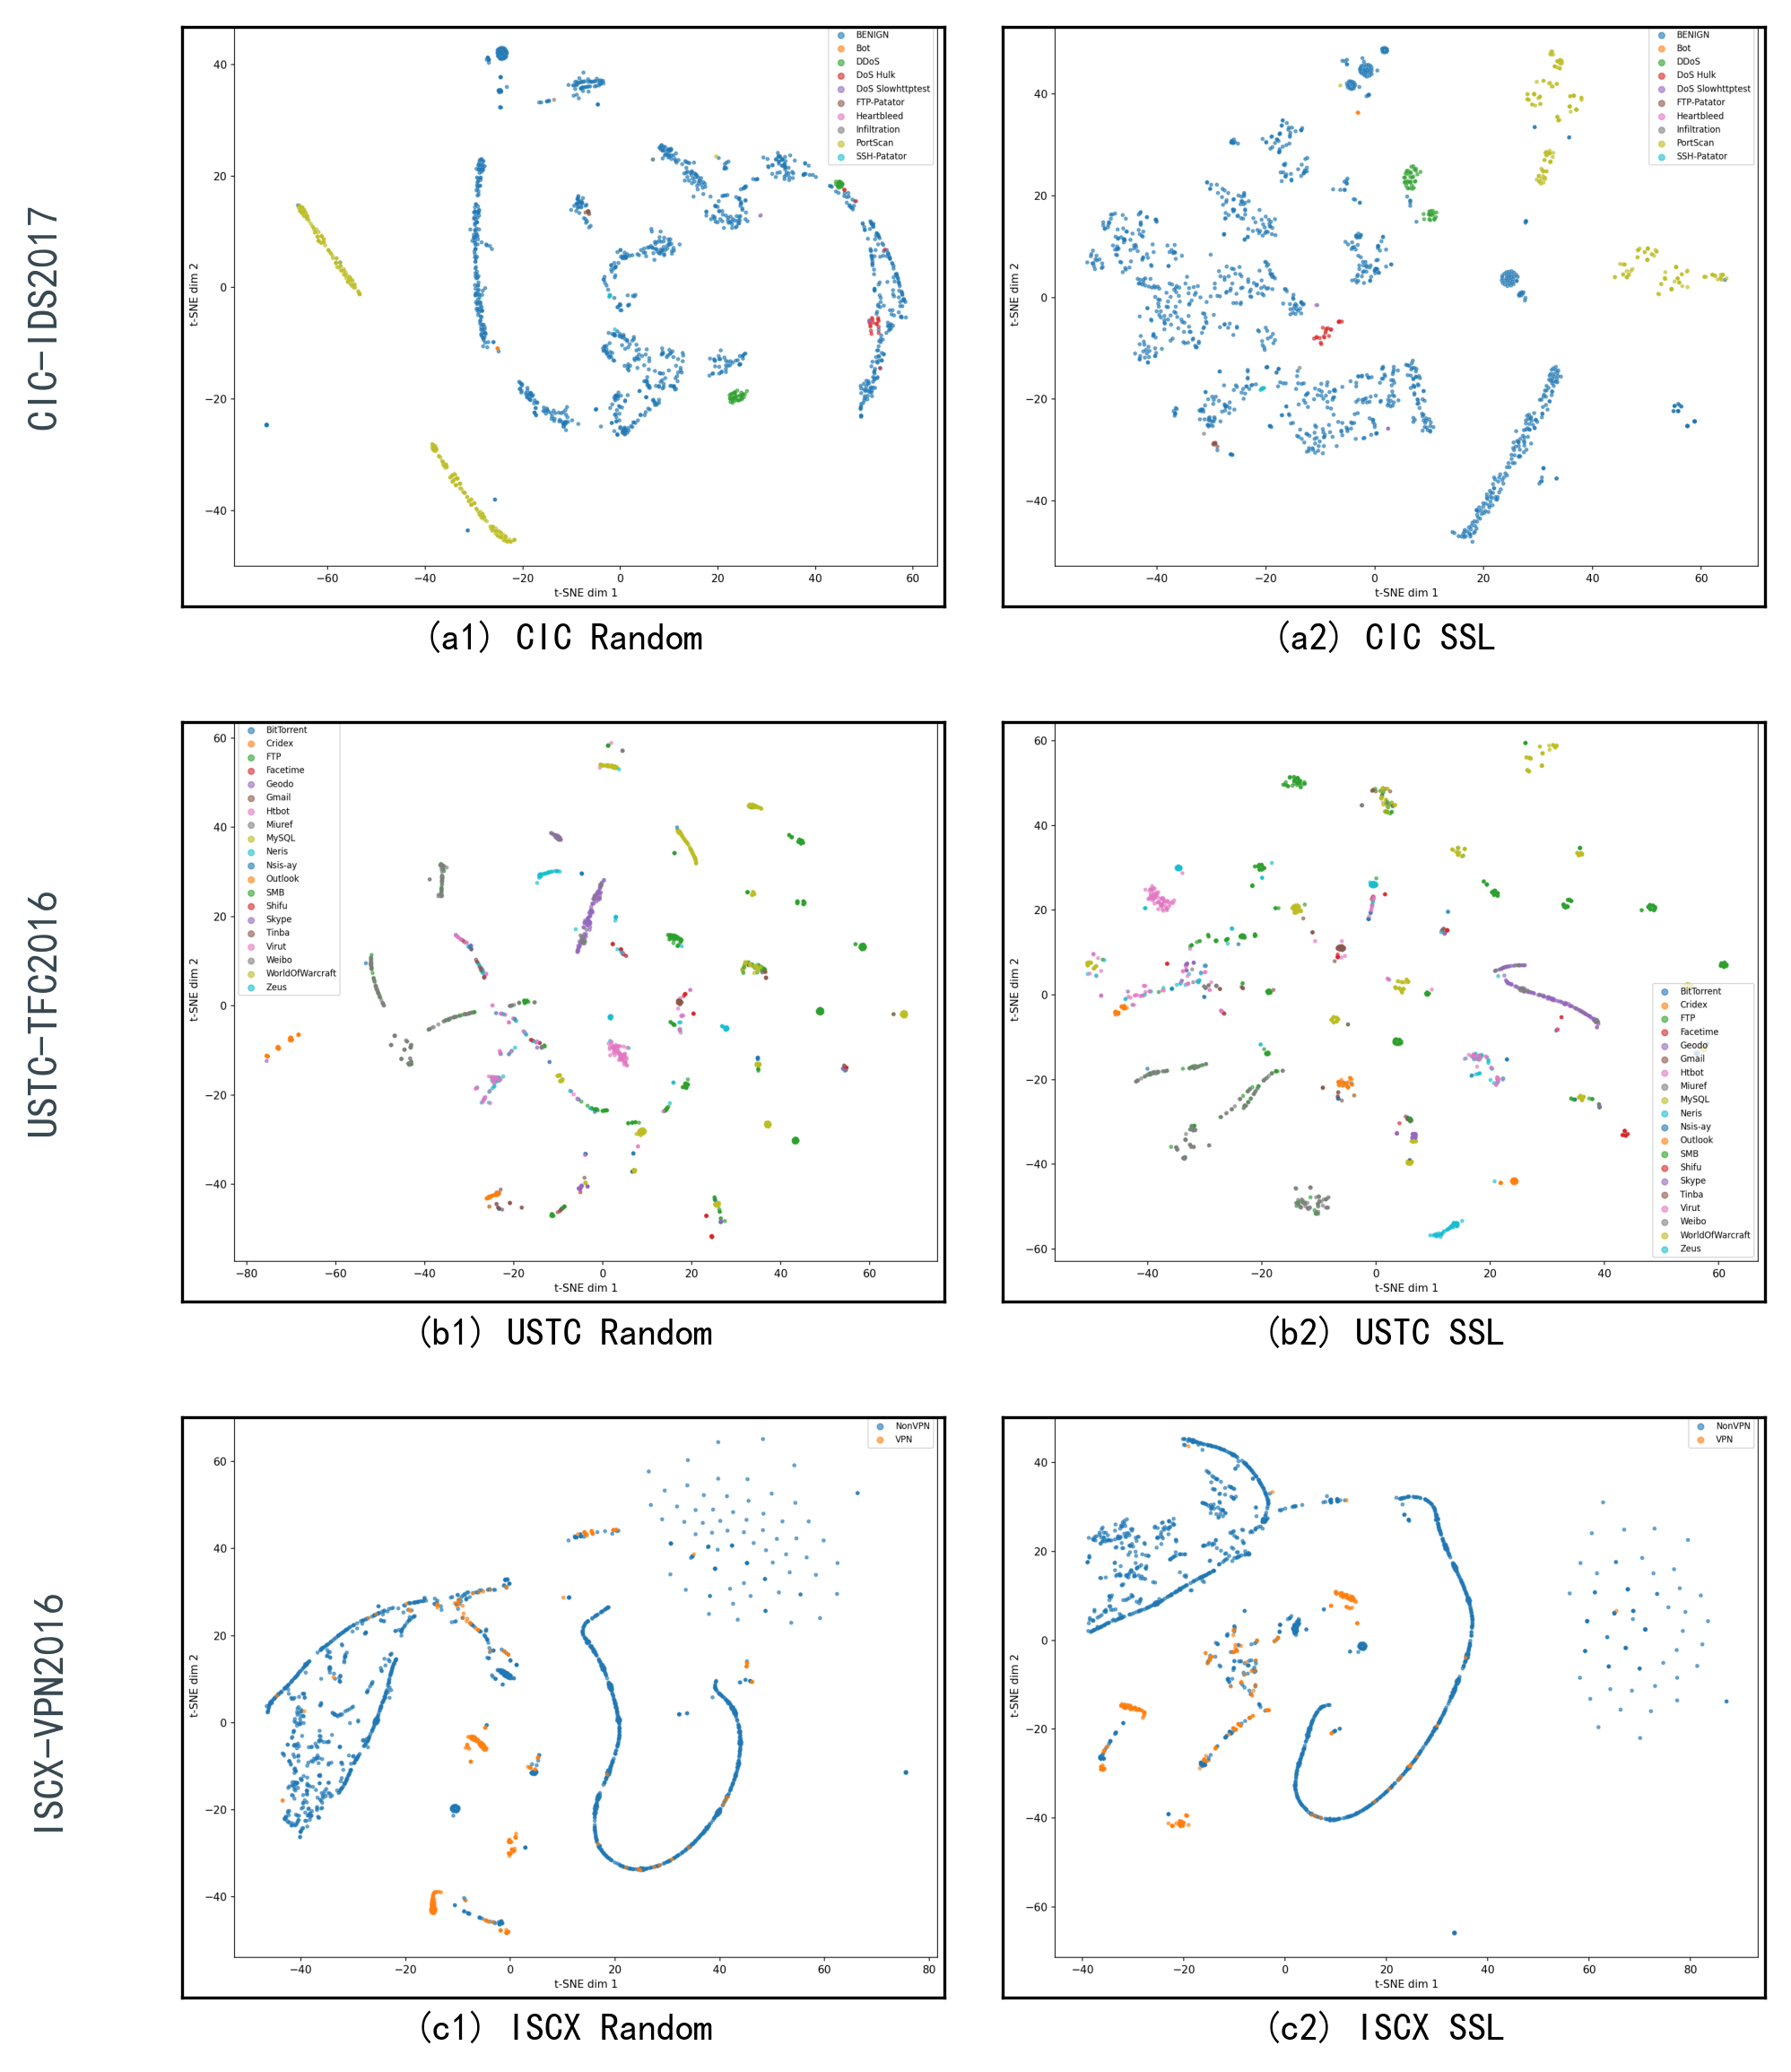
\includegraphics{figures/figA1_tsne.png}}
\caption{t-SNE projections (3 datasets $\times$ Random / SSL; subcaptions (a1)--(c2) at the same size as the figure caption).}
\label{fig:tsne_appx}
\end{figure}

\begin{figure}[htbp]
\centering
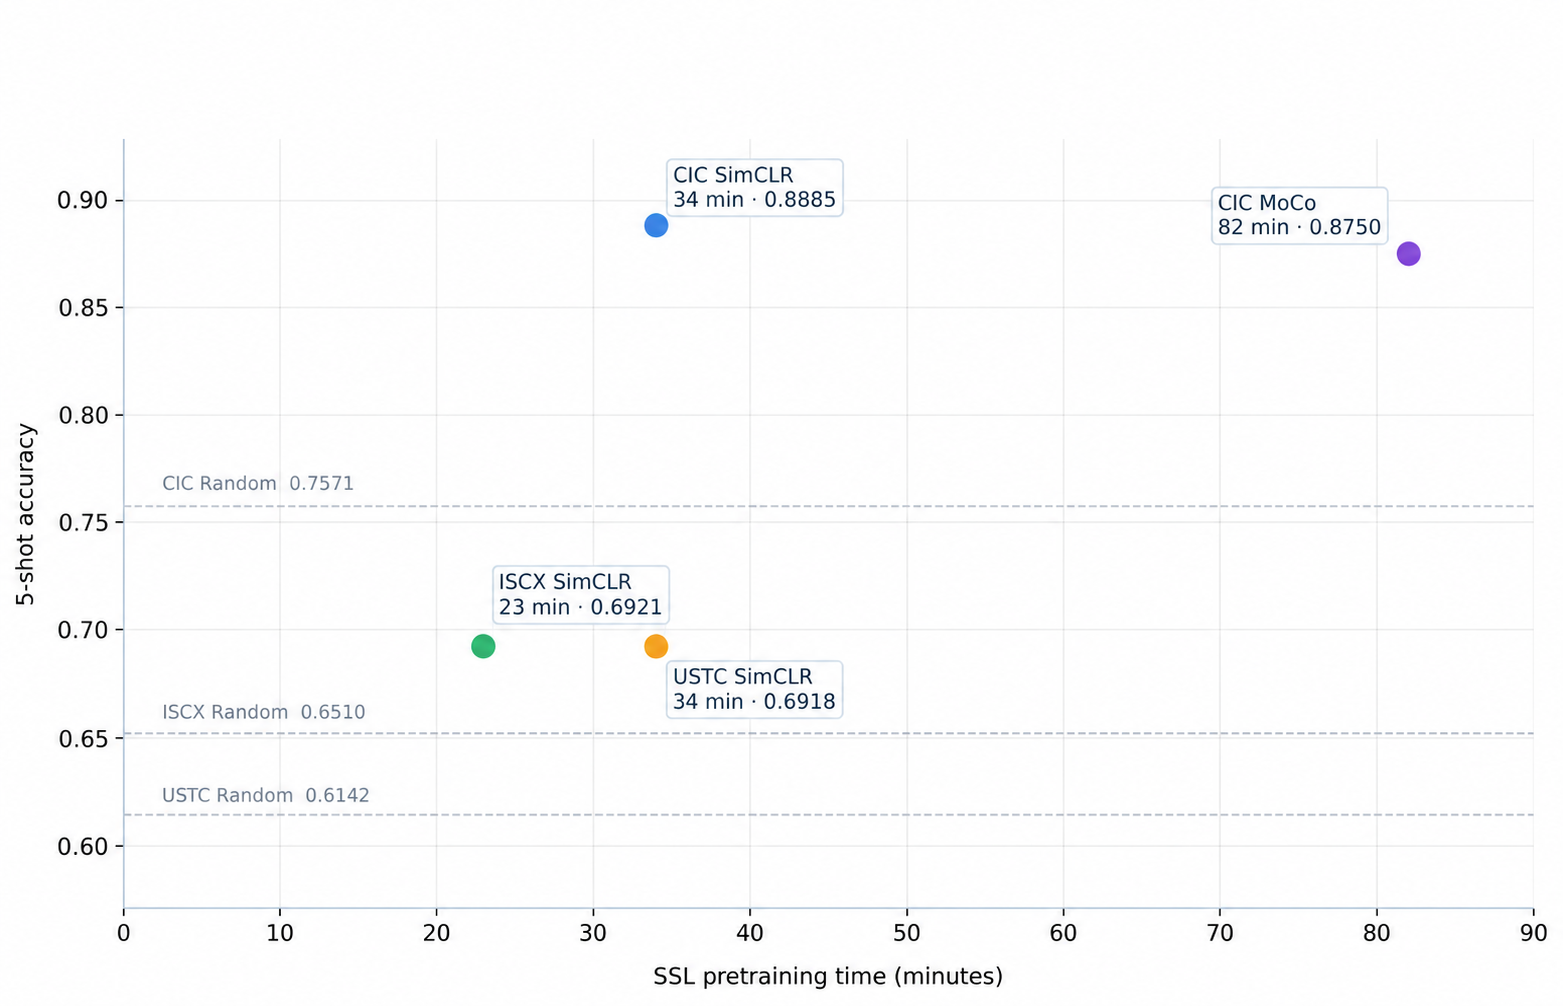
\includegraphics[width=\textwidth]{figures/fig8_ssl_efficiency.png}
\caption{SSL pretraining cost--benefit scatter.}
\label{fig:efficiency_appx}
\end{figure}

\begin{table}[H]
\centering
\small
\caption{Full $K$-shot scan ($3\ \text{seeds} \times 200\ \text{episodes}$; \textbf{note: this appendix table uses a smaller protocol than Table~\ref{tab:mainexp} ($5\ \text{seeds} \times 600\ \text{episodes}$)}; the $K=5$ row here is consistent with Table~\ref{tab:sslfamily} but differs from Table~\ref{tab:mainexp} by sample-size variance; cited in Section~\ref{sec:mainexp}).}
\label{tab:kshotscan}
\setlength{\tabcolsep}{4pt}
\begin{tabular}{cccccc}
\toprule
Dataset & K-shot & 1 & 3 & 5 & 10 \\
\midrule
\multirow{2}{*}{CIC-IDS2017}  & SSL    & 0.8521 & 0.8624 & 0.8700 & 0.8752 \\
                            & Random & 0.7728 & 0.7366 & 0.7115 & 0.6799 \\
                            & $\Delta$ (pp) & +7.93 & +12.58 & +15.85 & +19.53 \\
\midrule
\multirow{2}{*}{USTC-TFC2016} & SSL    & 0.6621 & 0.7258 & 0.7391 & 0.7525 \\
                            & Random & 0.6995 & 0.7376 & 0.7465 & 0.7498 \\
                            & $\Delta$ (pp) & $-3.74$ & $-1.18$ & $-0.74$ & +0.27 \\
\midrule
\multirow{2}{*}{ISCX-VPN2016} & SSL    & 0.6786 & 0.6407 & 0.6462 & 0.6443 \\
                            & Random & 0.6328 & 0.6266 & 0.6419 & 0.6484 \\
                            & $\Delta$ (pp) & +4.58 & +1.41 & +0.43 & $-0.41$ \\
\bottomrule
\end{tabular}
\end{table}

\begin{table}[H]
\small
\caption{SSL algorithm diversity (ProtoNet $N$-way $K$-shot, $3\ \text{seeds} \times 200\ \text{episodes}$, ISCX is 2-way; \textbf{note: this appendix table uses a smaller $3 \times 200$ protocol than Table~\ref{tab:mainexp}; absolute numbers therefore differ slightly from Table~\ref{tab:mainexp} but the ranking is preserved}; ranking discussed in Section~\ref{sec:sslalgo}).}
\label{tab:sslfamily}
\begin{adjustwidth}{-\extralength}{0cm}
\begin{tabularx}{\fulllength}{>{\raggedright\arraybackslash}X >{\raggedright\arraybackslash}X >{\centering\arraybackslash}X >{\centering\arraybackslash}X >{\centering\arraybackslash}X >{\centering\arraybackslash}X} 
\toprule
SSL algorithm & Paradigm & CIC-IDS2017 & USTC-TFC2016 & ISCX-VPN2016 & 3-dataset mean \\
\midrule
\textbf{SimCLR} & Contrastive (in-batch negatives) & \textbf{0.8700 $\pm$ 0.004} & \textbf{0.7391 $\pm$ 0.008} & \textbf{0.7026 $\pm$ 0.008} & \textbf{0.7706} \\
MoCo       & Contrastive (momentum queue)        & 0.8537 $\pm$ 0.002 & 0.6606 $\pm$ 0.006 & 0.6249 $\pm$ 0.012 & 0.7131 \\
BYOL       & Bootstrapping (EMA target)         & 0.8676 $\pm$ 0.001 & 0.6802 $\pm$ 0.004 & 0.6104 $\pm$ 0.010 & 0.7194 \\
SimSiam    & Bootstrapping (stop-gradient)      & 0.8465 $\pm$ 0.003 & 0.6592 $\pm$ 0.006 & 0.5573 $\pm$ 0.013 & 0.6877 \\
Embedding-MAE$\dagger$ & Reconstructive (embed.\ mask) & 0.7886 $\pm$ 0.003 & 0.6121 $\pm$ 0.005 & 0.5806 $\pm$ 0.011 & 0.6604 \\
\bottomrule
\end{tabularx}%
\end{adjustwidth}
\vspace{0.5ex}
\noindent\textit{Note: $\dagger$ Embedding-MAE (simplified version in this paper) $\neq$ the MAE of He et al.\ 2022; see Section~\ref{sec:sslalgo}.}
\end{table}

\begin{table}[H]
\centering
\small
\caption{Extended SimCLR heads comparison (MoCo / MatchingNet columns removed from Table~\ref{tab:mainexp} for compactness; full data restored here, 5 seeds $\times$ 600 episodes).}
\label{tab:sslheads}
\setlength{\tabcolsep}{4pt}
\begin{tabular}{ccccc}
\toprule
Dataset & Task & SimCLR + MoCo & SimCLR + MatchingNet & $\Delta_{\text{Proto-Match}}$ (pp) \\
\midrule
CIC-IDS2017   & 5-way 5-shot & 0.8750 $\pm$ 0.003 & 0.8760 $\pm$ 0.003 & $+1.25$ \\
USTC-TFC2016  & 5-way 5-shot & 0.5880 $\pm$ 0.005 & 0.6203 $\pm$ 0.005 & $+7.15$ \\
ISCX-VPN2016  & 2-way 5-shot & 0.6223 $\pm$ 0.003 & 0.6097 $\pm$ 0.003 & $+8.24$ \\
\bottomrule
\end{tabular}
\\[0.5ex]
\noindent\textit{Note: $\Delta_{\text{Proto-Match}}$ = (SimCLR + ProtoNet) $-$ (SimCLR + MatchingNet), i.e.\ the metric-learning gain over cosine attention. SimCLR $>$ MoCo by $+1.35$ pp on CIC (0.8885 vs 0.8750); MoCo is worse than Random on USTC/ISCX.}
\end{table}

\begin{table}[H]
\centering
\small
\caption{USTC per-class 5-shot accuracy (SSL vs Random, 5 seeds $\times$ 600 episodes; top 5 + bottom 5, 10 classes; cited in Section~\ref{sec:xdataset}).}
\label{tab:ustcpc}
\setlength{\tabcolsep}{4pt}
\begin{tabular}{cccc}
\toprule
Application class & SSL & Random & $\Delta$ (pp) \\
\midrule
\multicolumn{4}{c}{\textit{--- SSL top 5 (SSL strongest) ---}} \\
Outlook & 0.9906 & 0.9920 & $-0.14$ \\
WorldOfWarcraft & 0.9822 & 0.9999 & $-1.77$ \\
Tinba & 0.9280 & 0.3932 & \textbf{+53.48} \\
Skype & 0.9021 & 0.9142 & $-1.21$ \\
Facetime & 0.8822 & 0.8891 & $-0.69$ \\
\midrule
\multicolumn{4}{c}{\textit{--- SSL bottom 5 (SSL weakest) ---}} \\
BitTorrent & 0.5196 & 0.5845 & $-6.49$ \\
Neris & 0.5153 & 0.3855 & \textbf{+12.98} \\
Gmail & 0.5120 & 0.5164 & $-0.44$ \\
Miuref & 0.5024 & 0.3135 & \textbf{+18.89} \\
Nsis-ay & 0.5007 & 0.2413 & \textbf{+25.94} \\
\bottomrule
\end{tabular}
\end{table}

\begin{table}[H]
\centering
\small
\caption{Open-set FSL evaluation (CIC / USTC, 3 seeds $\times$ 200 ep; cited in Section~\ref{sec:soc}).}
\label{tab:openset}
\setlength{\tabcolsep}{4pt}
\begin{tabular}{cccccc}
\toprule
Dataset & Scenario A & Scenario B & Scenario C & Scenario B & Scenario C \\
 & closed-set acc & AUROC & AUROC & conf gap & conf gap \\
\midrule
CIC-IDS2017  & 0.8261 & \textbf{0.9127 $\pm$ 0.004} & 0.8285 $\pm$ 0.002 & \textbf{0.51} & 0.29 \\
USTC-TFC2016 & 0.8736 & 0.8022 $\pm$ 0.003 & 0.7202 $\pm$ 0.008 & 0.07 & 0.07 \\
\bottomrule
\end{tabular}
\end{table}

%% ----------------------------------------------------------------
%% References
%% ----------------------------------------------------------------
\begin{adjustwidth}{-\extralength}{0cm}
\reftitle{References}

\begin{thebibliography}{999}

\bibitem{cisco2024threat}
Cisco Systems, \textit{Cybersecurity Threat Trends: AI, Encryption and the Rise of Encrypted Traffic}, Cisco Cybersecurity Report, 2024. \\
\url{https://www.cisco.com/c/en/us/products/security/cybersecurity-reports.html}



\bibitem{liu2019fsnet}
C. Liu, L. He, G. Xiong, Z. Cao, Z. Li, FS-Net: A flow sequence network for encrypted traffic classification, in: \textit{IEEE INFOCOM 2019 - IEEE Conference on Computer Communications}, 2019, pp. 1171--1179. \\
\url{https://doi.org/10.1109/INFOCOM.2019.8737507}



\bibitem{zhao2023yatc}
R. Zhao, M. Zhan, X. Deng, Y. Wang, Y. Wang, G. Gui, Z. Xue, Yet another traffic classifier: A masked autoencoder based traffic transformer with multi-level flow representation, in: \textit{Proceedings of the AAAI Conference on Artificial Intelligence}, Vol. 37, No. 4, 2023, pp. 5420--5427. \\
\url{https://doi.org/10.1609/aaai.v37i4.25674}



\bibitem{lin2022etbert}
X. Lin, G. Xiong, G. Gou, Z. Li, J. Shi, J. Yu, ET-BERT: A contextualized datagram representation with pre-training transformers for encrypted traffic classification, in: \textit{Proceedings of the ACM Web Conference 2022 (WWW '22)}, 2022. \\
\url{https://doi.org/10.1145/3485447.3512217}



\bibitem{zhang2023tfegnn}
H. Zhang, L. Yu, X. Xiao, Q. Li, F. Mercaldo, X. Luo, Q. Liu, TFE-GNN: A temporal fusion encoder using graph neural networks for fine-grained encrypted traffic classification, in: \textit{Proceedings of the ACM Web Conference 2023 (WWW '23)}, 2023, pp. 2066--2075. \\
\url{https://doi.org/10.1145/3543507.3583227}



\bibitem{dhinakar2026survey}
N. Joseph Pramod Dhinakar, K. Ramani, Deep learning approaches to encrypted traffic classification: A comprehensive survey, \textit{AIP Conference Proceedings} 3371 (2026) 030006. \\
\url{https://doi.org/10.1063/5.0312319}



\bibitem{liu2025iot}
Y. Liu, Y. Guo, Enhancing intrusion detection for IoT and sensor networks through semantic analysis and self-supervised embeddings, \textit{Sensors} 25 (22) (2025) 7074. \\
\url{https://doi.org/10.3390/s25227074}



\bibitem{wang2024netmamba}
T. Wang, X. Xie, W. Wang, C. Wang, Y. Zhao, Y. Cui, NetMamba: Efficient network traffic classification via pre-training unidirectional mamba, in: \textit{2024 IEEE 32nd International Conference on Network Protocols (ICNP)}, 2024. \\
\url{https://doi.org/10.1109/ICNP61940.2024.10858569}



\bibitem{lekhac2020contrastive}
P.H. Le-Khac, G. Healy, A.F. Smeaton, Contrastive representation learning: A framework and review, \textit{IEEE Access} 8 (2020) 193907--193934. \\
\url{https://doi.org/10.1109/ACCESS.2020.3031549}



\bibitem{jing2021ssl}
L. Jing, Y. Tian, Self-supervised visual feature learning with deep neural networks: A survey, \textit{IEEE Transactions on Pattern Analysis and Machine Intelligence} 43 (11) (2021) 4037--4058. \\
\url{https://doi.org/10.1109/TPAMI.2020.2992393}



\bibitem{dong2025sslreview}
W. Dong, J. Yu, X. Lin, G. Gou, G. Xiong, Deep learning and pre-training technology for encrypted traffic classification: A comprehensive review, \textit{Neurocomputing} 617 (2025) 128444. \\
\url{https://doi.org/10.1016/j.neucom.2024.128444}



\bibitem{wang2020fsl}
Y. Wang, Q. Yao, J.T. Kwok, L.M. Ni, Generalizing from a few examples: A survey on few-shot learning, \textit{ACM Computing Surveys} 53 (3) (2020) 1--34. \\
\url{https://doi.org/10.1145/3386252}



\bibitem{chen2020simclr}
T. Chen, S. Kornblith, M. Norouzi, G. Hinton, A simple framework for contrastive learning of visual representations, in: \textit{Proceedings of the 37th International Conference on Machine Learning (ICML)}, PMLR 119, 2020, pp. 1597--1607. \\
\url{https://proceedings.mlr.press/v119/chen20j.html}



\bibitem{he2020moco}
K. He, H. Fan, Y. Wu, S. Xie, R. Girshick, Momentum contrast for unsupervised visual representation learning, in: \textit{Proceedings of the IEEE/CVF Conference on Computer Vision and Pattern Recognition (CVPR)}, 2020, pp. 9729--9738. \\
\url{https://doi.org/10.1109/CVPR42600.2020.00975}



\bibitem{grill2020byol}
J.-B. Grill, F. Strub, F. Altch\'e, et al., Bootstrap your own latent: A new approach to self-supervised learning, in: \textit{Advances in Neural Information Processing Systems (NeurIPS)}, Vol. 33, 2020. \\
\url{https://proceedings.neurips.cc/paper/2020/hash/f3ada80d5c4ee70142b17b8192b2958e-Abstract.html}



\bibitem{chen2021simsiam}
X. Chen, K. He, Exploring simple siamese representation learning, in: \textit{Proceedings of the IEEE/CVF Conference on Computer Vision and Pattern Recognition (CVPR)}, 2021, pp. 15750--15758. \\
\url{https://doi.org/10.1109/CVPR46437.2021.01549}



\bibitem{he2022mae}
K. He, X. Chen, S. Xie, Y. Li, P. Doll\'ar, R. Girshick, Masked autoencoders are scalable vision learners, in: \textit{Proceedings of the IEEE/CVF Conference on Computer Vision and Pattern Recognition (CVPR)}, 2022, pp. 16000--16009. \\
\url{https://doi.org/10.1109/CVPR52688.2022.01553}



\bibitem{snell2017protonet}
J. Snell, K. Swersky, R.S. Zemel, Prototypical networks for few-shot learning, in: \textit{Advances in Neural Information Processing Systems (NeurIPS)}, Vol. 30, 2017, pp. 4078--4088. \\
\url{https://proceedings.neurips.cc/paper/2017/hash/cb8da6767461f2812ae4290eac7cbc42-Abstract.html}



\bibitem{vinyals2016matching}
O. Vinyals, C. Blundell, T. Lillicrap, K. Kavukcuoglu, D. Wierstra, Matching networks for one shot learning, in: \textit{Advances in Neural Information Processing Systems (NeurIPS)}, Vol. 29, 2016, pp. 3630--3638. \\
\url{https://proceedings.neurips.cc/paper/2016/hash/90e1357833654983612fb05e3ec9148c-Abstract.html}



\bibitem{finn2017maml}
C. Finn, P. Abbeel, S. Levine, Model-agnostic meta-learning for fast adaptation of deep networks, in: \textit{Proceedings of the 34th International Conference on Machine Learning (ICML)}, PMLR 70, 2017, pp. 1126--1135. \\
\url{https://proceedings.mlr.press/v70/finn17a.html}



\bibitem{sung2018relationnet}
F. Sung, Y. Yang, L. Zhang, T. Xiang, P.H.S. Torr, T.M. Hospedales, Learning to compare: Relation network for few-shot learning, in: \textit{Proceedings of the IEEE Conference on Computer Vision and Pattern Recognition (CVPR)}, 2018, pp. 1199--1208. \\
\url{https://doi.org/10.1109/CVPR.2018.00131}



\bibitem{hang2023flowmae}
Z. Hang, Y. Lu, Y. Wang, Y. Xie, Flow-MAE: Leveraging masked autoencoder for accurate, efficient and robust malicious traffic classification, in: \textit{Proceedings of the 26th International Symposium on Research in Attacks, Intrusions and Defenses (RAID '23)}, 2023. \\
\url{https://doi.org/10.1145/3607199.3607206}



\bibitem{chang2026ictmeta}
C. Chang, Y. Li, S. Seneviratne, X. Cai, ICT-META: In-context aware few-shot learner for encrypted traffic classification, \textit{IEEE Transactions on Machine Learning in Communications and Networking} 4 (2026) 733--743. \\
\url{https://doi.org/10.1109/TMLCN.2026.3685578}



\bibitem{li2025contrastivemeta}
Z. Li, J. Wang, Y.-F. Song, S.-H. Yue, Unlocking few-shot encrypted traffic classification: A contrastive-driven meta-learning approach, \textit{Electronics} 14 (21) (2025) 4245. \\
\url{https://doi.org/10.3390/electronics14214245}



\bibitem{zhao2026pretraincontrast}
L. Zhao, T. Wu, J. Yu, When pre-training meets contrast learning: Few-shot encrypted traffic classification with novelty detection, \textit{IEEE/ACM Transactions on Networking} 34 (2026). \\
\url{https://doi.org/10.1109/TON.2026.3674624}



\bibitem{qu2026sepSpace}
Y. Qu, C. Zheng, M. Liao, H. Ma, Y. Jiang, W. Wang, SepSpace: Payload-free open-set network traffic classification via supervised contrastive representation learning and prototype-radius rejection, \textit{Cybersecurity} 9 (2026) 204. \\
\url{https://doi.org/10.1186/s42400-026-00635-x}



\bibitem{golchin2024ssclids}
P. Golchin, N. Rafiee, M. Hajizadeh, A. Khalil, R. Kundel, R. Steinmetz, SSCL-IDS: Enhancing generalization of intrusion detection with self-supervised contrastive learning, in: \textit{2024 IFIP Networking Conference (IFIP Networking)}, 2024. \\
\url{https://ieeexplore.ieee.org/document/10619725}



\bibitem{jin2025mamlcl}
Y. Jin, J. Fang, Y. Gao, Few-shot encrypted traffic classification model incorporating MAML and contrastive learning, \textit{Journal of Shanghai University (Natural Science Edition)} 31 (4) (2025) 719--734. \\
\url{https://doi.org/10.23919/IFIPNetworking62109.2024.10619725}



\bibitem{rahaman2026review}
M. Rahaman, A. Mahmud, A. Abd Aziz, O.M.S. Abujawa, J.-J. Chin, A systematic literature review on data-efficient and adaptive learning techniques for encrypted traffic classification under modern protocols, \textit{Computers} 15 (5) (2026) 319. \\
\url{https://doi.org/10.3390/computers15050319}



\bibitem{yang2024clidssurvey}
Y. Yang, Contrastive learning for network intrusion detection: A comprehensive survey, in: \textit{Proceedings of the 2024 2nd International Conference on Computer, Internet of Things and Smart City (CloTSC)}, 2024. \\
\url{https://doi.org/10.1145/3731867.3731894}



\bibitem{atitallah2024iot}
S. Ben Atitallah, M. Driss, W. Boulila, A. Koubaa, Strengthening network intrusion detection in IoT environments with self-supervised learning and few-shot learning, \textit{arXiv preprint} (2024) arXiv:2406.02636. \\
\url{https://arxiv.org/abs/2406.02636}



\bibitem{lu2026cdtf}
Z. Lu, M. Chen, S. Cui, B. Zhao, Y. Zheng, A contrastive dual-task framework for few-shot traffic classification in IoT networks, \textit{Sensors} 26 (11) (2026) 3471. \\
\url{https://doi.org/10.3390/s26113471}



\bibitem{xian2017zeroshot}
Y. Xian, B. Schiele, Z. Akata, Zero-shot learning --- the good, the bad and the ugly, in: \textit{Proceedings of the IEEE Conference on Computer Vision and Pattern Recognition (CVPR)}, 2017, pp. 4582--4591. \\
\url{https://doi.org/10.1109/CVPR.2017.328}



\bibitem{sharafaldin2018cicids}
I. Sharafaldin, A.H. Lashkari, A.A. Ghorbani, Toward generating a new intrusion detection dataset and intrusion traffic characterization, in: \textit{Proceedings of the 4th International Conference on Information Systems Security and Privacy (ICISSP)}, 2018, pp. 108--116. \\
\url{https://doi.org/10.5220/0006639801080116}



\bibitem{wang2017ustc}
W. Wang, M. Zhu, X. Zeng, X. Ye, Y. Sheng, Malware traffic classification using convolutional neural network for representation learning, in: \textit{2017 International Conference on Information Networking (ICOIN)}, 2017, pp. 712--717. \\
\url{https://doi.org/10.1109/ICOIN.2017.7899588}



\bibitem{draper2016iscx}
G. Draper-Gil, A.H. Lashkari, M.S.I. Mamun, A.A. Ghorbani, Characterization of encrypted and VPN traffic using time-related features, in: \textit{Proceedings of the 2nd International Conference on Information Systems Security and Privacy (ICISSP)}, 2016, pp. 407--414. \\
\url{https://doi.org/10.5220/0005740704070414}



\bibitem{tang2022netconv}
S. Tang, X. Chen, Network traffic classification based on 1D convolutional network (NetConv), in: \textit{2022 IEEE 8th International Conference on Computer and Communications (ICCC)}, 2022, pp. 1637--1643. \\
\url{https://www.mdpi.com/1424-8220/25/22/7074}



\bibitem{montazeri2021dohbrw}
S. MontazeriShatoori, L. Cerf, B. Roberson, U. Javidan, G. Varghese, DoHBrw-2020: A comprehensive dataset of malicious and benign DoH traffic captures (version 1.0), Stratosphere IPS Lab, 2021. \\
\url{https://doi.org/10.1109/DASC-PICom-CBDCom-CyberSciTech49142.2020.00026}

\end{thebibliography}


\PublishersNote{}
\end{adjustwidth}
\end{document}
